% Options for packages loaded elsewhere
\PassOptionsToPackage{unicode}{hyperref}
\PassOptionsToPackage{hyphens}{url}
\PassOptionsToPackage{dvipsnames,svgnames,x11names}{xcolor}
%
\documentclass[
  singlecolumn]{report}

\usepackage{amsmath,amssymb}
\usepackage{iftex}
\ifPDFTeX
  \usepackage[T1]{fontenc}
  \usepackage[utf8]{inputenc}
  \usepackage{textcomp} % provide euro and other symbols
\else % if luatex or xetex
  \usepackage{unicode-math}
  \defaultfontfeatures{Scale=MatchLowercase}
  \defaultfontfeatures[\rmfamily]{Ligatures=TeX,Scale=1}
\fi
\usepackage[]{libertinus}
\ifPDFTeX\else  
    % xetex/luatex font selection
\fi
% Use upquote if available, for straight quotes in verbatim environments
\IfFileExists{upquote.sty}{\usepackage{upquote}}{}
\IfFileExists{microtype.sty}{% use microtype if available
  \usepackage[]{microtype}
  \UseMicrotypeSet[protrusion]{basicmath} % disable protrusion for tt fonts
}{}
\makeatletter
\@ifundefined{KOMAClassName}{% if non-KOMA class
  \IfFileExists{parskip.sty}{%
    \usepackage{parskip}
  }{% else
    \setlength{\parindent}{0pt}
    \setlength{\parskip}{6pt plus 2pt minus 1pt}}
}{% if KOMA class
  \KOMAoptions{parskip=half}}
\makeatother
\usepackage{xcolor}
\usepackage[top=30mm,left=20mm,heightrounded]{geometry}
\setlength{\emergencystretch}{3em} % prevent overfull lines
\setcounter{secnumdepth}{-\maxdimen} % remove section numbering
% Make \paragraph and \subparagraph free-standing
\ifx\paragraph\undefined\else
  \let\oldparagraph\paragraph
  \renewcommand{\paragraph}[1]{\oldparagraph{#1}\mbox{}}
\fi
\ifx\subparagraph\undefined\else
  \let\oldsubparagraph\subparagraph
  \renewcommand{\subparagraph}[1]{\oldsubparagraph{#1}\mbox{}}
\fi


\providecommand{\tightlist}{%
  \setlength{\itemsep}{0pt}\setlength{\parskip}{0pt}}\usepackage{longtable,booktabs,array}
\usepackage{calc} % for calculating minipage widths
% Correct order of tables after \paragraph or \subparagraph
\usepackage{etoolbox}
\makeatletter
\patchcmd\longtable{\par}{\if@noskipsec\mbox{}\fi\par}{}{}
\makeatother
% Allow footnotes in longtable head/foot
\IfFileExists{footnotehyper.sty}{\usepackage{footnotehyper}}{\usepackage{footnote}}
\makesavenoteenv{longtable}
\usepackage{graphicx}
\makeatletter
\def\maxwidth{\ifdim\Gin@nat@width>\linewidth\linewidth\else\Gin@nat@width\fi}
\def\maxheight{\ifdim\Gin@nat@height>\textheight\textheight\else\Gin@nat@height\fi}
\makeatother
% Scale images if necessary, so that they will not overflow the page
% margins by default, and it is still possible to overwrite the defaults
% using explicit options in \includegraphics[width, height, ...]{}
\setkeys{Gin}{width=\maxwidth,height=\maxheight,keepaspectratio}
% Set default figure placement to htbp
\makeatletter
\def\fps@figure{htbp}
\makeatother
\newlength{\cslhangindent}
\setlength{\cslhangindent}{1.5em}
\newlength{\csllabelwidth}
\setlength{\csllabelwidth}{3em}
\newlength{\cslentryspacingunit} % times entry-spacing
\setlength{\cslentryspacingunit}{\parskip}
\newenvironment{CSLReferences}[2] % #1 hanging-ident, #2 entry spacing
 {% don't indent paragraphs
  \setlength{\parindent}{0pt}
  % turn on hanging indent if param 1 is 1
  \ifodd #1
  \let\oldpar\par
  \def\par{\hangindent=\cslhangindent\oldpar}
  \fi
  % set entry spacing
  \setlength{\parskip}{#2\cslentryspacingunit}
 }%
 {}
\usepackage{calc}
\newcommand{\CSLBlock}[1]{#1\hfill\break}
\newcommand{\CSLLeftMargin}[1]{\parbox[t]{\csllabelwidth}{#1}}
\newcommand{\CSLRightInline}[1]{\parbox[t]{\linewidth - \csllabelwidth}{#1}\break}
\newcommand{\CSLIndent}[1]{\hspace{\cslhangindent}#1}

\usepackage{cancel}
\makeatletter
\makeatother
\makeatletter
\makeatother
\makeatletter
\@ifpackageloaded{caption}{}{\usepackage{caption}}
\AtBeginDocument{%
\ifdefined\contentsname
  \renewcommand*\contentsname{Table of contents}
\else
  \newcommand\contentsname{Table of contents}
\fi
\ifdefined\listfigurename
  \renewcommand*\listfigurename{List of Figures}
\else
  \newcommand\listfigurename{List of Figures}
\fi
\ifdefined\listtablename
  \renewcommand*\listtablename{List of Tables}
\else
  \newcommand\listtablename{List of Tables}
\fi
\ifdefined\figurename
  \renewcommand*\figurename{Figure}
\else
  \newcommand\figurename{Figure}
\fi
\ifdefined\tablename
  \renewcommand*\tablename{Table}
\else
  \newcommand\tablename{Table}
\fi
}
\@ifpackageloaded{float}{}{\usepackage{float}}
\floatstyle{ruled}
\@ifundefined{c@chapter}{\newfloat{codelisting}{h}{lop}}{\newfloat{codelisting}{h}{lop}[chapter]}
\floatname{codelisting}{Listing}
\newcommand*\listoflistings{\listof{codelisting}{List of Listings}}
\makeatother
\makeatletter
\@ifpackageloaded{caption}{}{\usepackage{caption}}
\@ifpackageloaded{subcaption}{}{\usepackage{subcaption}}
\makeatother
\makeatletter
\@ifpackageloaded{tcolorbox}{}{\usepackage[skins,breakable]{tcolorbox}}
\makeatother
\makeatletter
\@ifundefined{shadecolor}{\definecolor{shadecolor}{rgb}{.97, .97, .97}}
\makeatother
\makeatletter
\makeatother
\makeatletter
\makeatother
\ifLuaTeX
  \usepackage{selnolig}  % disable illegal ligatures
\fi
\IfFileExists{bookmark.sty}{\usepackage{bookmark}}{\usepackage{hyperref}}
\IfFileExists{xurl.sty}{\usepackage{xurl}}{} % add URL line breaks if available
\urlstyle{same} % disable monospaced font for URLs
\hypersetup{
  pdftitle={Better Causal Diagrams (DAGS) for Cultural Evolutionary Research},
  pdfauthor={Joseph A. Bulbulia},
  colorlinks=true,
  linkcolor={blue},
  filecolor={Maroon},
  citecolor={Blue},
  urlcolor={Blue},
  pdfcreator={LaTeX via pandoc}}

\title{Better Causal Diagrams (DAGS) for Cultural Evolutionary Research}
\author{Joseph A. Bulbulia}
\date{}

\begin{document}
\maketitle
\ifdefined\Shaded\renewenvironment{Shaded}{\begin{tcolorbox}[sharp corners, borderline west={3pt}{0pt}{shadecolor}, interior hidden, enhanced, frame hidden, boxrule=0pt, breakable]}{\end{tcolorbox}}\fi

\listoffigures
\listoftables
\hypertarget{abstract}{%
\section{Abstract}\label{abstract}}

\hypertarget{introduction}{%
\section{Introduction}\label{introduction}}

Correlation is not causation. However, across many human sciences,
persistent confusion in the analysis and reporting of correlations has
limited scientific progress. The direction of causation frequently runs
in the opposite direction to the direction of manifest correlations.
This problem is widely known. Nevertheless, many human scientists report
manifest correlations using hedging language. Making matters worse,
widely adopted strategies for confounding control fail
(\protect\hyperlink{ref-mcelreath2020}{McElreath 2020}), suggesting a
``causality crisis'' (\protect\hyperlink{ref-bulbulia2022}{Bulbulia
2022}). Addressing the causality crisis is arguably among the human
science's most pressing tasks.

When integrated into methodologically rigorous workflows, causal
directed acyclic graphs (``DAGs'', or ``causal diagramms'') can be
powerful tools for clarifying causality.\footnote{The term ``DAG'' is
  unfortunate because not all directed acyclic graphs are causal. For a
  graph to be causal it must satisfy the conditions of markov
  factorisation (see Appendix A).} A system of formal mathematical
proofs underpins their design. This brings confidence. No formal
mathematical training is required to use them. This makes them
accessible. However, causal inference relies on assumptions. Causal
diagrams are methods for encoding such assumptions. Where assumptions
are unwarrented, causal diagrams may deceive. For example, when
researchers lack time-series data, unbiased causal effect estimates are
generally not warrented. Thus, cross-sectional researchers who deploy
causal diagrams use them as scaffolding to uphold shaky assumptions.
Ideally, however, causal diagrams would serve as circuit breakers,
halting such misapplications in their tracks.

In this article, I introduce a suite of techniques for constructing
causal diagrams aimed at minimising unwarranted use. These are referred
to as \emph{chronologically causal graphs}. I offer a comprehensive
tutorial on applying these to cultural evolutionary research.

There are many excellent introductions to causal diagrams
(\protect\hyperlink{ref-rohrer2018}{Rohrer 2018};
\protect\hyperlink{ref-hernuxe1nmarobinsjm2020}{Hernán, MA, Robins JM
2020a}; \protect\hyperlink{ref-cinelli2022}{Cinelli, Forney, and Pearl
2022}; \protect\hyperlink{ref-barrett2021}{Barrett 2021};
\protect\hyperlink{ref-mcelreath2020}{McElreath 2020};
\protect\hyperlink{ref-greenland1999}{Greenland, Pearl, and Robins
1999}; \protect\hyperlink{ref-suzuki2020}{Suzuki, Shinozaki, and
Yamamoto 2020}; \protect\hyperlink{ref-pearl2009}{Pearl
2009}).\footnote{One of the best resources is Miguel Hernan's free
  course, here:
  \url{https://pll.harvard.edu/course/causal-diagrams-draw-your-assumptions-your-conclusions}.}.
One may reasonably ask whether another introduction adds clutter. The
approach I present here adds value in five ways.

This article is organised into five distinct sections.

In \textbf{Part 1}, I elucidate the role of causal diagrams in the
context of counterfactual, or ``potential'' outcomes. I challenge the
perception of causal inference as merely a facet of manifest data
science, arguing instead for its role within counterfactual data
science. This approach allows us to quantitatively address `What if?'
scenarios, which are crucial for evaluating causal claims. We will
review the counterfactual basis of quantitative causal inference, which
must be understood before attempting to use causal diagrams.

\textbf{Part 2} is devoted to an exploration of the four basic forms of
confounding. I introduce chronological causal diagrams and demonstrate
how they can help strategise for confounding control. Despite covering
familiar material, the emphasis here is on temporal order and its
benefits for understanding conditions that enable or inhibit causal
identification amidst confounding. I will also touch upon how these
diagrams can bring clarity to widely used concepts such as interaction,
mediation, and repeated measures longitudinal data, whose basis is
frequently misunderstood. I also discuss the inadequacy of commonly used
modelling techniques, such as multilevel modelling and structural
equation modelling, which fall short of the demands of counterfactual
data.

In \textbf{Part 3}, I discuss the advantages of collecting repeated
measures data for at least three waves, as highlighted by chronological
causal diagrams. This discussion provides guidance for how cultural
evolutionary researchers may record history in the present for future
inferential use.

\textbf{Part 4} discusses selection bias in a three-wave panel. The
chronological causal diagrams clarify the importance of adequate
sampling and longitudinal retention.

Lastly, in \textbf{Part 5}, I confront the issue of measurement error as
encountered in a three-wave panel. Again, chronological causal diagrams
guide the discussion, underscoring the need for reliable measures and
routes for confounding from correlated and directed measurement errors.
This section will be particularly beneficial to researchers in
comparative cultural research, especially those employing composite
scales.

Throughout, it is the application of chronologically ordered causal
diagrams in the setting of counterfactual data science that illuminates
both effective research strategies and their limitations.

\hypertarget{part-1.-the-three-fundamental-identifiability-assumption-for-counterfactual-data-science}{%
\section{Part 1. The three fundamental identifiability assumption for
counterfactual data
science}\label{part-1.-the-three-fundamental-identifiability-assumption-for-counterfactual-data-science}}

Before we can answer causal questions we must first understand how to
ask them. In this section I review key concepts and identification
assumptions.

\hypertarget{the-fundamental-problem-of-causal-inference}{%
\subsection{The fundamental problem of causal
inference}\label{the-fundamental-problem-of-causal-inference}}

We claim that \(A\) causes \(Y\) if altering \(A\) would have influenced
the outcome of \(Y\) (\protect\hyperlink{ref-hume1902}{Hume 1902};
\protect\hyperlink{ref-lewis1973}{Lewis 1973}). This claim requires
counterfactual reasoning, as the causal effect is conceptualised through
the contrast between the world as it is, and the world as it could have
been. Our objective in ``causal inference'' is to quantify this
contrast.

Consider an observed correlation between cultural beliefs in Big Gods
and social complexity. Suppose we hope to quantify the magnitude of the
causal effect of belief in Big Gods on social complexity. We say that
beliefs in Big Gods is the ``exposure'' or ``treatment,'' represented by
\(A\). We say that social complexity is the outcome, denoted by \(Y\).
For the time being, we assume the exposure, outcome, and units
(cultures) are well-defined (these assumptions will be revisited later).

In order to evaluate causality, we must establish two counterfactual (or
``potential'') outcomes for each culture within a population:

\begin{itemize}
\tightlist
\item
  \(Y_i(a = 1)\): The social complexity of culture \(i\) under belief in
  Big Gods. This outcome is counterfactual for cultures where
  \(A_i = 0\).
\item
  \(Y_i(a = 0)\): The social complexity of culture \(i\) without belief
  in Big Gods. This outcome is counterfactual for cultures where
  \(A_i = 1\).\footnote{The counterfactual outcome under exposure
    \(A = a\) can be denoted in several ways, such as \(Y(a)\),
    \(Y^{a}\), and \(Y_a\), with \(Y(a)\) being our chosen notation.
    These exposures are assumed to be exhaustive for the sake of
    simplicity.}
\end{itemize}

We can define the causal effect of belief in Big Gods on social
complexity for a given culture as the difference between potential
outcomes \(Y_i(a)\) under \emph{both} exposure levels (\(A_i = 1\) and
\(A_i = 0\)).

\[
\text{Causal Effect of Belief in Big Gods}_i = Y_i(1) - Y_i(0) 
\]

To determine causality, we need a contrast between two states of the
world, yet any culture can only experience one. The causal effect is not
identified in the data. This problem is known as ``the fundamental
problem of causal inference'' (\protect\hyperlink{ref-rubin1976}{Rubin
1976}; \protect\hyperlink{ref-holland1986}{Holland 1986}). It arises
because our observable data only provide partial evidence for
quantifying causal contrasts. Inferring counterfactual contrasts thus
becomes a type of \emph{missing data problem}
(\protect\hyperlink{ref-westreich2015}{Westreich et al. 2015};
\protect\hyperlink{ref-edwards2015}{Edwards, Cole, and Westreich 2015}).

\hypertarget{counterfactual-data-science-approach-to-estimate-average-causal-effects}{%
\subsubsection{Counterfactual data-science approach to estimate average
causal
effects}\label{counterfactual-data-science-approach-to-estimate-average-causal-effects}}

Individual-level causal effects are typically unobservable, however, we
can estimate average causal effects. We achieve this by comparing the
average outcome across the population under two different conditions -
when all units are exposed (to a certain level of treatment) and when
none are exposed (to another level). This contrast can be expressed on a
difference scale.\footnote{Note that the difference in average
  expectations is equivalent to the average of the differences in
  expectations.}

The average treatment effect (ATE) can be represented by the equation:

\[
ATE = E[Y(a)] - E[Y(a*)]
\]

Remember, each unit is only observable under one level of exposure,
therefore individual-level causal effects are generally not identifiable
from the data. Nonetheless, if the three fundamental identification
principles can be credibly assumed, we can infer these average (or
``marginal'') contrasts from the data to calculate average (or marginal)
causal contrasts. Note that we are not restricted to binary exposures.
We can derive contrasts between two different levels of a multinomial or
continuous exposure by defining the exposure levels we wish to compare
as \(A = a\) and \(A = a^*\).

\hypertarget{identification-assumption-1-causal-consistency}{%
\subsection{Identification assumption 1: Causal
consistency}\label{identification-assumption-1-causal-consistency}}

\textbf{The problem: missing counterfactual outcomes}: we need both
observed and unobserved potential outcomes to evaluate the average
treatment effects (ATE):

\[
ATE = \bigg(E[Y(1)|A = 1]_{\text{observed}} + E[Y(1)|A = 0]_{\text{unobserved}}\bigg) - \bigg(E[Y(0)|A = 0]_{\text{observed}}  + E[Y(0)|A = 1]_{\text{unobserved}}\bigg)
\]

\textbf{The solution: Causal Consistency}: this assumption permits us to
equate potential outcomes under exposure \(Y_i(A_i=a)\) with their
observed counterparts \(Y_i^{observed}|A=a\). Using this, we represent
observed outcomes as follows:

\[
Y^{observed}_i = 
\begin{cases} 
Y_i(~a^*) & \text{if } A_i = a* \\
Y_i(~a~) & \text{if } A_i = a
\end{cases}
\]

In practice, this assumption allows us to substitute observed outcomes
for the missing counterfactual outcomes under hypothetical exposures,
thus enabling us to estimate causal contrasts from observed data. That
is, where the assumption of causal consistency is tenable, we say that
the missing counterfactual outcomes under hypothetical exposures are
equal to the observed outcomes under realised exposures.

\textbf{The foil: non-interference}: a condition for causal consistency
is the assumption of non-interference between units. This means that the
potential outcome for unit \(i\) under treatment \(a_i\) should be
independent of the treatment assignment to any other unit \(j\):

\[
Y_i(a_i, a_j) = Y_i(a_i, a'_j)
\]

for all \(a_j, a'_j\). Violations of this condition can occur when there
are dependencies in the data, such as in social networks. For example,
the efficacy of a vaccine may typically depend on the frequency and
density of vaccination in the population, violating the non-interference
assumption.

\textbf{The work-around}: where there are \(K\) different versions of
treatment \(A\) that individuals receive, we may consistently estimate
causal effects under the assumptions of ``treatment variation
irrelevance.'' If the effects if the variations of the treatment are
independent of the counterfactual outcomes under such treatments, that
is, if there is no confounding for \(K\)'s effect on \(Y\) given
measured confounders \(L\) such that:

\[
K \coprod Y(k) | L
\]

or equivalently

\[
Y(k) \coprod K | L
\]

Then we can use \(A\) as a ``coarsened indicator'' to estimate the
causal effect of the multiple versions of treatment \(K\) on \(Y(k)\)
(\protect\hyperlink{ref-vanderweele2009}{Tyler J. VanderWeele 2009},
\protect\hyperlink{ref-vanderweele2018}{2018};
\protect\hyperlink{ref-vanderweele2013}{Tyler J. VanderWeele and Hernan
2013}).

\textbf{The spoiler for this work-around}: these assumptions of
``treatment variation irrelevance'' can be problematic, particularly
when the interventions (the \(K\) treatment versions) are not
well-defined, or if we cannot accurately assess the conditional
independence assumption. Hence, when defining treatments and outcomes
for estimating causal effects, the importance of precision cannot be
overstated. (I will return to this topic in Part 3.)

\textbf{The essential task: recovering missing counterfactual
observations}: Ultimately, causal consistency provides a theoretical
framework enabling us to bridge the gap between what is observed and
what remains unseen in our data. It equips us to translate actual
observations into unobserved counterfactual outcomes, enabling us -- by
assumptions -- to compute the causal contrasts required for quantifying
average treatment effects. Despite its utility, that we are missing
missing half of observations remains a persistent challenge. Filling
this gap requires the interplay of further assumptions, such as
exchangeability and positivity to which we turn next.

\hypertarget{identification-assumption-2-exchangeability}{%
\subsection{Identification Assumption 2:
Exchangeability}\label{identification-assumption-2-exchangeability}}

Exchangeability, the second identification assumption, underpins the
mechanism of treatment assignment. Specifically, it stipulates that,
conditional on observed covariates, treatment assignment is independent
of potential outcomes. This assumption confers ``exchangeability''
between individual units across exposure and contrast conditions.
Conceptually, if we could swap units between these conditions, and if
both the consistency and positivity assumption were also satisfied, then
the distribution of potential outcomes would remain unchanged. In other
words, we require exchangeability because we require balance between
treatment conditions in the confounders potentially affecting the
outcome. Denote \(L\) as a measured covariate that ensures conditional
independence; we then express exchangeability as:

\[
Y(a) \coprod  A|L \quad \text{or equivalently} \quad A \coprod  Y(a)|L
\]

When exchangeability holds, conditional on measured covariates, we can
express the average treatment effect (ATE) as follows:

\[
ATE = E[Y(a^*)|L = l] - E[Y(a)|L = l]
\] It is important to note that causal diagrams are tools that were
developed to evaluate the exchangeability assumption. While they can be
useful for assessing the causal consistency assumption and the
positivity assumption, their primary utility lies in clarifying
conditions for consistent causal effect estimation by either including
or omitting covariates to ensure conditional exchangeability
(\protect\hyperlink{ref-hernuxe1nmarobinsjm2020}{Hernán, MA, Robins JM
2020a}).

\hypertarget{identification-assumption-3-positivity}{%
\subsection{Identification Assumption 3:
Positivity}\label{identification-assumption-3-positivity}}

The positivity assumption, the third identification assumption, posits a
non-zero probability of receiving or not receiving the exposure within
each level of the covariates. In other words, within every stratum of
covariates, the probability of each exposure value is greater than zero.
Mathematically, we express this as:

\[
0 < \Pr(A=a|L)<1, ~ \forall a \in A, ~ \forall l \in L
\]

Without satisfying the positivity assumption, causal inference becomes
problematic since we cannot envisage causal contrasts without the
possibility for interventions
(\protect\hyperlink{ref-westreich2010}{Westreich and Cole 2010}).

This assumption is subject to two types of violations:

\begin{enumerate}
\def\labelenumi{\arabic{enumi}.}
\item
  \textbf{Random Non-Positivity}: Here, the causal effect is imaginable,
  but some observations are missing within our data, which could
  theoretically exist. For instance, with a continuous exposure, there
  will be absent realisations on the number line because of its infinite
  nature. Yet, we can still use statistical models to estimate causal
  contrasts. Importantly, random non-positivity is the only
  identifiability assumption that we can verify with data. While our
  focus here is not in guiding researchers on data modelling, it is
  worth noting that applied researchers must verify and report any
  violation of random non-positivity in their data.
\item
  \textbf{Deterministic Non-Positivity}: Here, the causal effect is
  inconceivable. A classic example is estimating the causal effect of a
  hysterectomy in biological males, which naturally violates
  deterministic non-positivity due to biological constraints. We cannot
  compute causal contrasts for inconceivable interventions.
\end{enumerate}

\hypertarget{the-difficulty-of-satisfying-causal-consistency-and-positivity-assumptions-when-considering-historical-dynamics.}{%
\subsection{The difficulty of satisfying causal consistency and
positivity assumptions when considering historical
dynamics.}\label{the-difficulty-of-satisfying-causal-consistency-and-positivity-assumptions-when-considering-historical-dynamics.}}

Three critical assumptions underpin our capacity to extract significant
causal conclusions from data: causal consistency, exchangeability, and
positivity. Meeting these is challenging given the qualities of human
cultural histories.

Consider the Protestant Reformation. Martin Luther's reformation in the
16th century led to the establishment of Protestantism. Many have argued
that Protestantism caused social, cultural, and economic changes in
those societies where it took hold (see:
(\protect\hyperlink{ref-weber1905}{Weber 1905},
\protect\hyperlink{ref-weber1993}{1993};
\protect\hyperlink{ref-swanson1967}{Guy E. Swanson 1967};
\protect\hyperlink{ref-swanson1971}{Guy E. Swanson 1971};
\protect\hyperlink{ref-basten2013}{Basten and Betz 2013}), for an
overview see: (\protect\hyperlink{ref-becker2016}{Becker, Pfaff, and
Rubin 2016})).

Suppose we are interested in estimating the Average Treatment Effect
(ATE) of the Reformation. In this scenario, \(A = a*\) denotes the
adoption of Protestantism. We compare this effect with remaining
Catholic, represented as \(A = a\). We assume economic development is
well-defined. We define the outcome as GDP a century after a country
predominantly turns Protestant, compared with remaining Catholic,
\(Y_i(a^*) - Y_i(a)\). While we cannot identify this effect for a single
country, if the basic assumptions are met, we can estimate
\(\frac{1}{n} \sum_i^{n} Y_i(a*) - Y_i(a)\) and

\[ATE_{\textnormal{economic~development}} = E[Y(\textnormal{Became~Protestant}) - Y(\textnormal{Remained~Catholic})]\]

Consider the challenges we might have in satisfying ourselves of the
assumptions required for causal inference.

\textbf{Causal Consistency}: The Reformation occurred differently across
Europe. We must consider the ``Protestant vs Catholic treatment''
(\(a*\) or \(a\)) as consistent across these varied contexts. In
England, Protestantism was closely tied to the monarchy
(\protect\hyperlink{ref-collinson2007}{Collinson 2007}). In Germany,
Martin Luther's teachings emphasised individual faith and scripture
interpretation, which supported economic development by promoting
literacy (\protect\hyperlink{ref-gawthrop1984}{Gawthrop and Strauss
1984}). There is considerable heterogeneity in the ``Protestant
exposure,'' There is also ample scope for interference: 16th century
societies were interconnected through trade, diplomacy, and warfare.
Thus, the religious decisions of one society and their economic effects
were unlikely to be independent of the others' decisions and economic
effects.

\textbf{Exchangeability}: to compute causal effect estimates the
potential outcomes must be independent of treatment assignment given
measured covariates. Variables such as political stability or
educational attainment could simultaneously influence the likelihood of
a society adopting Protestantism and its level of economic progression.
If these potential confounders remain unadjusted for, the causal effect
of the Reformation on economic development could be falsely estimated.
Obtaining valid measures even for events as recent as the reformation is
challenging.

\textbf{Positivity}: This assumption requires that every unit at every
level of measured confounders has a non-zero probability of receiving
both treatments. However, it is unclear under which conditions 16th
century Spain could have been randomly assigned to Protestantism,
challenging the estimation of an Average Treatment Effect
(\protect\hyperlink{ref-nalle1987}{Nalle 1987}).

A possibly more meaningful credible measure of effect is arguably the
Average Treatment Effect in the Treated (ATT):

\[ATT = E[(Y(a*)- Y(a))|A = a*,L]\]

Here, ATT represents the expected difference in economic success for
cultures that became Protestant compared with the expected economic
success if those cultures had not become Protestant, conditional on
measured confounders \(L\), among the exposed (\(A = a^*\)). To estimate
this contrast, we would need to match Protestant cultures with
comparable non-protestant cultures. Whether matching is conceptually
plausible is a matter for historians and philosophers to consider.

Setting aside these conceptual challenges, there are significant
difficulties in meeting the requirements for the causal consistency,
exchangeability, and positivity assumptions. Assuming we can meet these
assumptions and resolve any questions about the measurement of variables
inducing an association between exposure and outcomes, we can then use
causal diagrams to assess the exchangeability assumption of no
unmeasured confounding.

\hypertarget{summary-part-1}{%
\subsection{Summary Part 1}\label{summary-part-1}}

Causal inference is a process that involves comparing two potential
outcomes by manipulating an intervention. This requires posing a ``What
if?'' question. For questions to have meaning, it is crucial to clearly
define both the intervention being imposed and the potential effects it
could engender.

Following this, it is important to understand, and then satisfy, the
assumptions needed to derive this hypothetical quantity -- the causal
contrast -- from the data. There are three essential assumptions: causal
consistencym which posits that the variation of treatment is irrelevant,
positivity, which asserts that the intervention is not deterministically
confined within the strata being compared, and exchangeability, which
requires no unmeasured confounders. Causal diagrams were developed to
assess the exchangeability assumption, but it is crucial to understand
that the tool -- and so its application -- is situated in a broader
setting of counterfactual data science.

\hypertarget{part-2.-chronologically-ordered-causal-diagrams}{%
\subsection{Part 2. Chronologically Ordered Causal
Diagrams}\label{part-2.-chronologically-ordered-causal-diagrams}}

\hypertarget{background-concepts-and-conventions}{%
\subsection{Background: Concepts and
Conventions}\label{background-concepts-and-conventions}}

To use causal diagrams, it is crucial to understand the following
concepts and conventions:

\begin{enumerate}
\def\labelenumi{\arabic{enumi}.}
\item
  \textbf{Nodes and Edges}: Nodes represent variables or events in a
  causal system, whereas edges denote the relationships between these
  variables.
\item
  \textbf{Directed and Undirected Edges}: Directed edges, marked by
  arrows, represent a causal influence from one variable to another.
  Undirected edges suggest an association or correlation without clear
  causality.
\item
  \textbf{Ancestors and Descendants}: A variable is an ancestor of
  another if it directly or indirectly influences it in the graph.
  Conversely, a variable is a descendant if it is influenced by another
  variable.
\item
  \textbf{Confounding Variables}: These are factors that influence both
  the exposure and the outcome, potentially distorting the observed
  relationship between them. In a causal graph, confounding variables
  are depicted as common ancestors of both cause and effect nodes.
\item
  \textbf{Control of Confounding by the Modified Disjunctive Cause
  Criterion}: VanderWeele's Modified Disjunctive Cause Criterion (MDCC)
  provides practical guidance for controlling for confounding. According
  to this criterion, a distinct variable that can reduce or remove the
  distortion caused by confounding variables is deemed a confounder when
  adjusted for
  (\protect\hyperlink{ref-vanderweele2019a}{\textbf{vanderweele2019a?}}).
  This criterion offers three essential directives:

  \begin{enumerate}
  \def\labelenumii{\alph{enumii}.}
  \item
    Control for any variable that causes the exposure, the outcome, or
    both.
  \item
    Control for any proxy for an unmeasured variable that is a shared
    cause of both exposure and outcome.
  \item
    Define an instrumental variable as a variable associated with the
    exposure but does not influence the outcome independently, except
    through the exposure. Exclude any instrumental variable that is not
    a proxy for an unmeasured confounder from the confounder set.
  \end{enumerate}
\item
  \textbf{D-Separation}: Paths in a causal graph show potential routes
  of influence between nodes. A path is blocked, or d-separated, if a
  node on it halts the transmission of influence. Two variables are
  d-separated if every path between them is blocked; otherwise, they are
  d-connected. The concept of d-separation is critical in the analysis
  of causal diagrams. It provides a method for determining whether any
  set of variables blocks the pathway from a set of variables \(X\) to a
  set \(Y\). Understanding this allows us to identify the conditions
  under which variables are independent, hence crucial in our assessment
  of causal relationships.
\item
  \textbf{Compatibility}: If two variables are d-separated given a
  third, the two variables are independent conditional on the third.
  Understanding compatibility is fundamental in assessing the
  independence of variables within a causal framework. The concept
  allows us to determine if, given a certain set of observed variables,
  two other variables are conditionally independent. This is key in
  identifying and addressing potential confounding in observational
  studies.
\item
  \textbf{(Weak) Faithfulness}: If two variables are d-connected given a
  third, the two variables are expected to be associated conditional on
  the third. The concept of faithfulness is a key assumption in causal
  analysis, asserting that any dependence relationship implied by the
  joint distribution of all variables is also represented in the causal
  graph. This bridges the gap between statistical association and causal
  relation, allowing us to deduce from observational data the potential
  existence of a causal pathway.
\item
  \textbf{Markov Factorisation}: relates graph structure to joint
  probability distributions of the represented variables. Given a causal
  graph with nodes corresponding to variables \(X = (X_1, ..., X_n)\),
  the joint distribution \(P(X)\) factorises according to the graph if
  expressed as a product of conditional distributions for each node
  given its direct parents. In formula terms,
  \(P(X) = \prod_{i=1}^{n} P(X_i | \text{pa}_G(X_i))\), where
  \(\text{pa}_G(X_i)\) are the parent nodes of \(X_i\) in graph \(G\).
  The principle of Markov factorisation provides a bridge between the
  structure of the causal graph and the joint probability distribution
  of the variables. By demonstrating that each variable is conditionally
  independent of its non-descendants given its parents, it allows
  complex multivariate distributions to be broken down into simpler
  conditional ones.
\item
  \textbf{Back-Door Criterion}: Understanding and applying the Back-Door
  Criterion is essential for estimating causal effects from
  observational data. It provides a set of conditions under which the
  effect of a treatment on an outcome can be obtained by controlling for
  a specific set of variables. Hence, it guides the selection of
  variables for adjustment to avoid confounding, ensuring more accurate
  estimation of causal effects.\footnote{Note, there is also a
    Front-Door Criterion, which provides another way to estimate causal
    effects, even in the presence of unmeasured confounding variables.
    It relies on identifying a variable (or set of variables) that
    mediates the entire effect of the treatment on the outcome. To my
    knowledge, the front-door criterion is rarely used in practice.}
\end{enumerate}

\begin{enumerate}
\def\labelenumi{\arabic{enumi}.}
\setcounter{enumi}{9}
\item
  \textbf{Identification Problem}: the challenge of estimating the
  causal effect of a variable using observed data. Causal graphs were
  developed to address the identification problem.
\item
  \textbf{Acyclic}: Causal diagrams must be acyclic - they cannot
  contain feedback loops. More precisely: no variable can be an ancestor
  or descendant of itself. Therefore, in cases where repeated
  measurements are taken, nodes must be indexed by time. As mentioned,
  repeated measures time series data are almost always required to
  quantitatively estimate causal effects. In section 3 we consider how
  adding baseline measures of the outcome and exposure in a three wave
  repeated measures design greatly enhances causal estimation.
  Chronologically ordered causal diagrams will therefore typically
  benefit from time-indexing of their nodes.
\item
  \textbf{Total, Direct and Indirect Effects}: in the presence of
  mediating variables, it is useful to differentiate the total effect
  (the overall effect of a variable \(A\) on an outcome \(Y\)), direct
  effect (the effect of \(A\) on \(Y\) not via any mediator), and
  indirect effect (the effect of \(A\) on \(Y\) via mediator). We
  consider the assumptions of causal mediation below.
\item
  \textbf{Time-varying Confounding}: We say there is time-varying
  confounding when a time-varying confounder is also a mediator in the
  causal pathway between exposure and outcome. Controlling for such a
  confounder could lead to bias. Longitudinal methods such as marginal
  structural models or G-methods are typically required to handle
  time-varying confounding. We consider the challenge of time-varying
  confounding below.
\item
  \textbf{Statistical Model:} A statistical model is a mathematical
  formulation that captures the relationships between observable or
  latent variables. It establishes a framework that quantifies how
  changes in one variable correspond with changes in others. For
  instance, in Part 5, we discuss the \textbf{reflective model of
  psychometric measurement}. This model posits that observable variables
  (indicators) are derived from or influenced by an unobserved (latent)
  variable. The relationship is typically expressed as
  \(X_i = \lambda_i \eta + \varepsilon_i\), where \(X_i\) is an observed
  variable, \(\eta\) is the latent variable, \(\lambda_i\) is the factor
  loading of the \(i\)th indicator, and \(\varepsilon_i\) is the error
  term.
\item
  \textbf{Structural Model:} A structural model extends beyond
  statistical models by incorporating hypotheses about causal
  relationships between variables. While statistical models delineate
  observed associations, structural models aim to provide a deeper
  understanding of the mechanisms behind these associations. Causal
  diagrams depict structural models. They make explicit the assumed
  paths of causation. Statistical models alone do not determine causal
  structures (\protect\hyperlink{ref-wright1920}{Wright 1920},
  \protect\hyperlink{ref-wright1923}{1923};
  \protect\hyperlink{ref-pearl2018}{Pearl and Mackenzie 2018};
  \protect\hyperlink{ref-hernuxe1nmarobinsjm2020a}{Hernán, MA, Robins JM
  2020b}). Deducing causal relationships typically requires further
  assumptions or information beyond what is available in the statistical
  model itself.
\end{enumerate}

\hypertarget{variable-naming-conventions}{%
\subsubsection{Variable Naming
Conventions}\label{variable-naming-conventions}}

\textbf{Outcome}: Here, denoted by \(Y\). The outcome, the ``effect,''
should be clearly defined in any causal diagram. Instead of stating
``the causal effect of the Protestant Reformation on economic success,''
be specific, such as ``the +100 year effect on adjusted GDP after a
country transitioned to a Protestant majority.'' This approach can
reveal limitations or challenges of causal inference, including
conceptual incoherence, lack of relevance, or data deficiencies.

\textbf{Exposure or Treatment}: Here, denoted by \(A\). The exposure
must be clearly defined and must not violate deterministic
non-positivity. Understanding the intervention allows accurate
assessment of how outcomes might vary with different interventions.

\textbf{Measured Confounders}: Here, denoted by \(L\). Confounders are
variables that, when adjusted for, minimise or remove the non-causal
association between exposure \(A\) and outcome \(Y\). To simplify a
causal graph, variables with similar functions are often grouped under a
single symbol. For example, if \(\text{male} \to A, Y\) and
\(\text{age} \to A, Y\), we can say \(\bf{L} \to A, Y\), where
\(\bf{L}\) is a set that includes the variables \(\text{male}\) and
\(\text{age}\) (\$\{\textbackslash text\{male, age

\hypertarget{elemental-counfounds}{%
\section{Elemental counfounds}\label{elemental-counfounds}}

There are four elemental confounds
(\protect\hyperlink{ref-mcelreath2020}{McElreath 2020, 185}). Here, we
consider how chronological order in a causal diagram assists with
clarifying and addressign the identification problem.

\hypertarget{the-problem-of-confounding-by-common-cause}{%
\subsection{1. The problem of confounding by common
cause}\label{the-problem-of-confounding-by-common-cause}}

The problem of confounding by common cause arises when there is a
variable denoted by \(L\) that influences both the exposure, denoted by
\(A\) and the outcome, denoted by \(Y.\) Because \(L\) is a common cause
of \(A\) and \(Y\), \(L\) may create a statistical association between
\(A\) and \(Y\) that does not reflect a causal association. For example,
people who smoke may have yellow fingers. Suppose smoking causes cancer.
Because smoking (\(L\)) is a common cause of yellow fingers (\(A\)) and
cancer (\(Y\)), \(A\) and \(Y\) will be associated in the data. However,
intervening to change the colour of a person's fingers would not affect
cancer. There is confounding. The dashed red arrow in the graph indicate
bias arising from the open backdoor path from \(A\) to \(Y\) that
results from the common cause \(L\).

\begin{figure}

{\centering 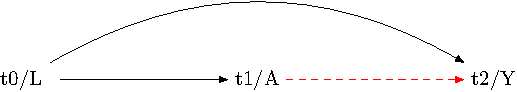
\includegraphics[width=0.8\textwidth,height=\textheight]{causal-dags_files/figure-pdf/fig-dag-common-cause-1.pdf}

}

\caption{\label{fig-dag-common-cause}Counfounding by common cause. The
dashed red arrow indicates bias arising from the open backdoor path from
A to Y.}

\end{figure}

\hypertarget{advice-attend-to-the-temporal-order-of-cauasality}{%
\subsection{Advice: attend to the temporal order of
cauasality}\label{advice-attend-to-the-temporal-order-of-cauasality}}

Confounding by a common cause can be addressed by adjusting for it.
Adjustment closes the backdoor path from the exposure to the outcome.
Typically we adjust through through regression, matching, inverse
probability of treatment weighting, and G-methods. (topics for another
tutorial.) Figure Figure~\ref{fig-dag-common-cause-solution} clarifies
that any confounding that is a cause of \(A\) and \(Y\) will precede
\(A\) (and so \(Y\)), because causes precede effects.

By indexing the the nodes on the graph, we can readily understand that
\textbf{confounding control typically requires time-series data.}

\begin{figure}

{\centering 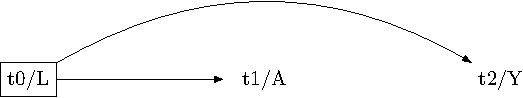
\includegraphics[width=0.8\textwidth,height=\textheight]{causal-dags_files/figure-pdf/fig-dag-common-cause-solution-1.pdf}

}

\caption{\label{fig-dag-common-cause-solution}Solution: adjust for
pre-exposure confounder.}

\end{figure}

\hypertarget{confounding-by-collider-stratification-conditioning-on-a-common-effect}{%
\subsection{2. Confounding by collider stratification (conditioning on a
common
effect)}\label{confounding-by-collider-stratification-conditioning-on-a-common-effect}}

Conditioning on a common effect occurs when a variable \(L\) is affected
by both the treatment \(A\) and an outcome \(Y\).

Suppose \(A\) and \(Y\) are initially independent, such that
\(A \coprod Y(a)\). Conditioning on the common effect \(L\) opens a
backdoor path between \(A\) and \(Y\), potentially inducing an
non-causal association. This occurs because \(L\) can provide
information about both \(A\) and \(Y\). Here is an example:

Let \(A\) denote the level of belief in Big Gods (with higher values
indicating stronger belief), \(Y\) denote the level of social
complexity, and \(L\) denote the level of economic trade. Now, suppose
that belief in Big Gods and social complexity are not causally linked.
However, suppose beliefs in Big Gods and social complexity influence
levels of economic trade. If we condition on economic trade without
attending to temporal order, we might find a statistical association
between belief in Big Gods and social complexity even though there is no
causal association.

To clarify, denote the observed associations as follows:

\begin{itemize}
\tightlist
\item
  \(P(A)\): Distribution of beliefs in Big Gods
\item
  \(P(Y)\): Distribution of social complexity
\item
  \(P(L)\): Distribution of economic trade
\end{itemize}

Without conditioning on \(L\), if \(A\) and \(Y\) are independent, we
have:

\[P(A, Y) = P(A)P(Y)\]

However, if we condition on \(L\) (which is a common effect of both
\(A\) and \(Y\)), we have:

\[P(A, Y | L) \neq P(A | L)P(Y | L)\]

The common effect \(L\), once conditioned on, creates an association
between \(A\) and \(Y\) that is not causal. This can mislead us into
believing there is a direct link between beliefs in Big Gods and social
complexity, even in the absence of such a link. If we only observe
\(A\), \(Y\), and \(L\) and compute correlations, without time-series
data measured on the units of analysis, we might erroneously conclude
that there is a causal relationship between \(A\) and \(Y\).\footnote{When
  \(A\) and \(Y\) are independent, the joint probability of \(A\) and
  \(Y\) is equal to the product of their individual probabilities:
  \(P(A, Y) = P(A)P(Y)\). However, when we condition on \(L\), the joint
  probability of \(A\) and \(Y\) given \(L\) is not necessarily equal to
  the product of the individual probabilities of \(A\) and \(Y\) given
  \(L\), hence the inequality \(P(A, Y | L) \neq P(A | L)P(Y | L)\).}

\begin{figure}

{\centering 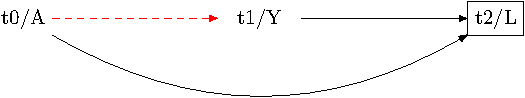
\includegraphics[width=0.8\textwidth,height=\textheight]{causal-dags_files/figure-pdf/fig-dag-common-effect-1.pdf}

}

\caption{\label{fig-dag-common-effect}Confounding by conditioning on a
collider. The dashed red arrow indicates bias arising from the open
backdoor path from A to Y.}

\end{figure}

\hypertarget{advice-attend-to-the-temporal-order-of-cauasality-showing-this-in-your-causal-graph-will-help-to-avoid-collider-bias}{%
\subsection{Advice: attend to the temporal order of cauasality, showing
this in your causal graph, will help to avoid collider
bias}\label{advice-attend-to-the-temporal-order-of-cauasality-showing-this-in-your-causal-graph-will-help-to-avoid-collider-bias}}

To address the problem of conditioning on a common effect, we should
generally ensure that all confounders \(L\) that are common causes of
the exposure \(A\) and the outcome \(Y\) are measured before the
occurence of the exposure \(A\), and furthermore that the exposure \(A\)
is measured before the occurence of the outcome \(Y\). If such temporal
order is preserved, \(L\) cannot be an effect of \(A\), and thus neither
of \(Y\). By measuring all relevant confounders before the exposure,
researchers can minimise the scope for collider confounding by
conditioning on a common effect. This rule is not absolute.\footnote{However,
  as indicated in Figure~\ref{fig-dag-descendent-solution}, it may be
  useful in certain circumstances to condition on a confounder that
  occurs after the outcome has occurred.}. In the case of the example
just described, we would require time-series data with accurate measures
in a sufficiently large sample of cultures prior to the introduction of
certain religious beliefs, and the cultures would need to be independent
of each other.\footnote{The independence of cultural units was at the
  centre of the study of comparative urban archeaology throughout from
  the late 19th
  (\protect\hyperlink{ref-decoulanges1903}{\textbf{decoulanges1903?}})
  and 20th century
  (\protect\hyperlink{ref-wheatley1971}{\textbf{wheatley1971?}}).
  Despite attention to this problem in recent work {[}e.g.
  (\protect\hyperlink{ref-watts2016}{\textbf{watts2016?}}){]}, there is
  arguably greater head-room for understanding the need for conditional
  independence of cultures in recent cultural evolutionary studies.
  Again, attending to temporal order of events is essential.}

\begin{figure}

{\centering 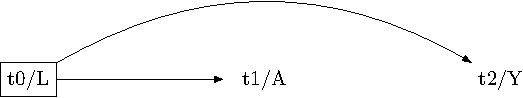
\includegraphics[width=0.8\textwidth,height=\textheight]{causal-dags_files/figure-pdf/fig-dag-common-effect-solution-1.pdf}

}

\caption{\label{fig-dag-common-effect-solution}Solution: time idexing of
confounders helps to avoid collider bias and maintain d-separation.}

\end{figure}

\hypertarget{m-bias-conditioning-on-a-collider-that-occurs-before-the-exposure-may-introduce-bias}{%
\subsection{M-bias: conditioning on a collider that occurs before the
exposure may introduce
bias}\label{m-bias-conditioning-on-a-collider-that-occurs-before-the-exposure-may-introduce-bias}}

Typically, indicators for confounders should included only if they are
known to be measured before their exposures ( exceptions described
below).

However, researchers should be also cautious about over-conditioning on
pre-exposure variables that are not associated with both the exposure
and confounder, as doing so can induce confounding. As shown in
Figure~\ref{fig-m-bias}, collider stratification may arise even if \(L\)
occurs before \(A\). This happens when \(L\) does not affect \(A\) or
\(Y\), but may be the descendent of a unmeasured variable that affects
\(A\) and another unmeasured variable that also affects \(Y\).
Conditioning on \(L\) in this scenario evokes what is called ``M-bias.''
If \(L\) is not a common cause of both \(A\) and \(Y\), or the effect of
a shared common cause, \(L\) should not be included in a causal model.
Figure~\ref{fig-m-bias} presents a case in which \(A \coprod Y(a)\) but
\(A \cancel{\coprod} Y(a)| L\). M-bias is another example of collider
stratification bias {[}see:
(\protect\hyperlink{ref-cole2010}{\textbf{cole2010?}}){]}

\begin{figure}

{\centering 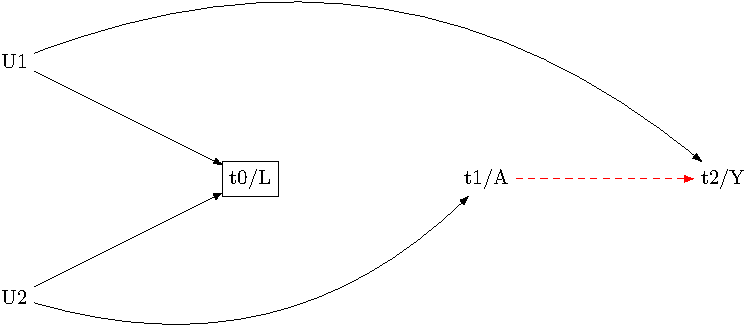
\includegraphics[width=0.8\textwidth,height=\textheight]{causal-dags_files/figure-pdf/fig-m-bias-1.pdf}

}

\caption{\label{fig-m-bias}M-bias: confounding control by including
previous measures of the outcome. The dashed red arrow indicates bias
arising from the open backdoor path from A to Y by conditioning on
pre-exposure variable L. The solution: do not condition on L.}

\end{figure}

\hypertarget{advice-adopt-a-modified-disjunctive-cause-criterion-for-confounding-control}{%
\subsection{Advice: adopt a modified disjunctive cause criterion for
confounding
control}\label{advice-adopt-a-modified-disjunctive-cause-criterion-for-confounding-control}}

Again, the modified disjunctive cause criterion will satisfy the
backdoor criterion in all cases, and reduce bias where this criterion
cannot be fully satisfied. Again:

\begin{verbatim}
a.  Control for any variable that causes the exposure, the outcome, or both.

b.  Control for any proxy for an unmeasured variable that is a shared cause of both exposure and outcome.

c.  Define an instrumental variable as a variable associated with the exposure but does not influence the outcome independently, except through the exposure. Exclude any instrumental variable that is not a proxy for an unmeasured confounder from the confounder set. [see: @vanderweele2020 page 441 and [@vanderweele2019a].]
\end{verbatim}

Of course, the difficulty is in determining which variables belong to
the desired set! This task can be facilitated by specialist knowledge
but cannot generally be ascertained from the data.

\hypertarget{the-pitfalls-of-conditioning-on-a-mediator}{%
\subsection{3 The pitfalls of conditioning on a
mediator}\label{the-pitfalls-of-conditioning-on-a-mediator}}

Conditioning on a mediator -- a variable that lies along the causal
pathway between the treatment and the outcome -- can distort the total
effect of the treatment on the outcome and potentially introduce bias.
To illustrate this, consider ``beliefs in Big Gods'' as the treatment
(\(A\)), ``social complexity'' as the outcome (\(Y\)), and ``economic
trade'' as the mediator (\(L\)).

In this scenario, the belief in Big Gods (\(A\)) has a direct impact on
economic trade (\(L\)), which subsequently influences social complexity
(\(Y\)). If we condition on economic trade (\(L\)), we could bias our
estimates of the overall effect of beliefs in Big Gods (\(A\)) on social
complexity (\(Y\)). This happens because conditioning on \(L\) can
downplay the direct effect of \(A\) on \(Y\), as it blocks the indirect
path through \(L\). This problem, known as mediator bias, is illustrated
in Figure~\ref{fig-dag-mediator}.

We might think that conditioning on a mediator does not introduce bias
under a null hypothesis (\(A\) does not cause \(Y\)), however this is
not the case. Consider a situation where \(L\) is a common effect of
both the exposure \(A\) and an unmeasured variable \(U\) linked to the
outcome \(Y\). In this scenario, including \(L\) may amplify the
association between \(A\) and \(Y\), even if \(A\) is not associated
with \(Y\) and \(U\) doesn't cause \(A\). This is represented in
Figure~\ref{fig-dag-descendent}.

So, unless one is specifically investigating mediation analysis, it is
usually not advisable to condition on a post-treatment variable. Paying
attention to chronology in the graph is crucial here: if we cannot
ensure that \(L\) is measured before \(A\) and \(A\) may affect \(L\),
including \(L\) in our model could result in mediator bias. This
scenario is presented in Figure~\ref{fig-dag-descendent}.

\begin{figure}

{\centering 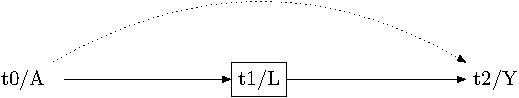
\includegraphics[width=0.8\textwidth,height=\textheight]{causal-dags_files/figure-pdf/fig-dag-mediator-1.pdf}

}

\caption{\label{fig-dag-mediator}Confounding by conditioning on a
mediator. The dashed black arrow indicates bias arising from partially
blocking the path between A and Y.}

\end{figure}

\hypertarget{advice-attend-to-the-temporal-order-of-causality}{%
\subsection{Advice: attend to the temporal order of
causality}\label{advice-attend-to-the-temporal-order-of-causality}}

To mitigate the issue of mediator bias, particularly when our focus is
on total effects, we should avoid conditioning on a mediator. This can
be achieved by ensuring that \(L\) occurs before the treatment \(A\) and
the outcome \(Y\) (A counter-example is presented in
Figure~\ref{fig-dag-descendent-solution-2}). Again we discover the
importance of explicitly stating the temporal ordering of our variables.
By including time indexing of all variables in our causal diagram and by
clearly labelling mediators, we reduce the potential for mediator bias
from over-conditioning.\footnote{Note that if \(L\) is associated with
  \(Y\) and cannot be caused by \(A\), conditioning on \(L\) will often
  enhance the precision of the estimate for the causal effect of \(A\)
  on \(Y\). This holds true even if \(L\) occurs after \(A\). However,
  the onus is on the researcher to show that the post-treatment factor
  cannot be a consequence of the exposure.}

\begin{figure}

{\centering 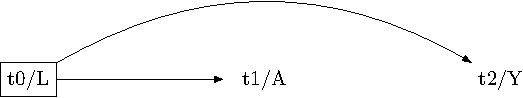
\includegraphics[width=0.8\textwidth,height=\textheight]{causal-dags_files/figure-pdf/fig-dag-mediator-solution-1.pdf}

}

\caption{\label{fig-dag-mediator-solution}Unless certain the exposure
cannot affect the confounder, ensure confounders are measured prior to
the exposure.}

\end{figure}

\hypertarget{conditioning-on-a-descendant}{%
\subsection{4. Conditioning on a
descendant}\label{conditioning-on-a-descendant}}

Say \(L\) is a cause of \(L^\prime\). According to Markov factorisation,
if we condition on \(L\), we partially condition on \(L^\prime\).

Consider how such conditioning might imperile causal estimation. Suppose
there is a confounder \(L^\prime\) that is caused by an unobserved
variable \(U\), and is affected by the treatment \(A\). Suppose further
that \(U\) causes the outcome \(Y\). In this scenario, as described in
Figure~\ref{fig-dag-descendent}, conditioning on \(L^\prime\), which is
a descendant of \(A\) and \(U\), can lead to a spurious association
between \(A\) and \(Y\) through the path \(A \to L^\prime \to U \to Y\).

\begin{figure}

{\centering 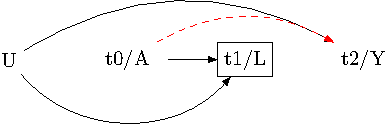
\includegraphics[width=0.8\textwidth,height=\textheight]{causal-dags_files/figure-pdf/fig-dag-descendent-1.pdf}

}

\caption{\label{fig-dag-descendent}Confounding by Descent: The red
dashed arrow illustrates the introduction of bias due to the opening of
a `backdoor' path between the exposure (A) and the outcome (Y) when
conditioning on a descendant of a confounder. This failure to maintain
d-separation in the association between the exposure and the outcome
leads to potential bias in the causal inference.}

\end{figure}

Again, the advice is clear: we should ensure that the (\(L^\prime\)) is
measured before the exposure (\(A\)). This solution is presented in
Figure~\ref{fig-dag-descendent-solution}.

\begin{figure}

{\centering 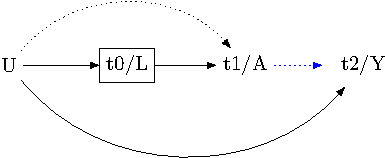
\includegraphics[width=0.8\textwidth,height=\textheight]{causal-dags_files/figure-pdf/fig-dag-descendent-solution-1.pdf}

}

\caption{\label{fig-dag-descendent-solution}Solution: again, ensure
temporal ordering in all measured variables. A and Y remain
d-separated.}

\end{figure}

Next consider how we may use a post-treatment descendent to reduce bias.
Suppose an unmeasured confounder \(U\) affects \(A\), \(Y\), and
\(L^\prime\) as presented in then adjusting for \(L^\prime\) may help to
reduce confounding caused by \(U\). This scenario is presented in
Figure~\ref{fig-dag-descendent-solution-2}. If we deploy the modified
disjunctive cause criterion for confounding control, we would ``include
as a covariate any proxy for an unmeasured variable that is a common
cause of both the exposure and the outcome''
(\protect\hyperlink{ref-vanderweele2019a}{\textbf{vanderweele2019a?}}).
We discover that although \(L^\prime\) may occur \emph{after} the
exposure, and indeed occur \emph{after} the outcome, we may condition on
it to reduce confounding because it is a proxy for an unmeasured common
cause of the exposure and the confounder. This expample shows that it
would be hasty to employ a rule that requires us to condition only on
pre-exposure (and indeed pre-outcome) variables.

\begin{figure}

{\centering 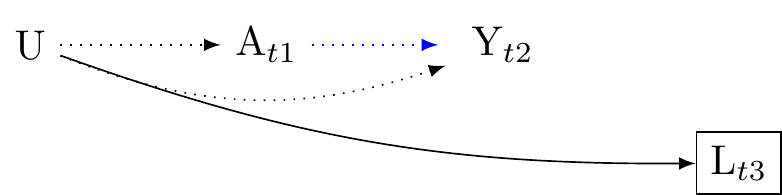
\includegraphics[width=0.8\textwidth,height=\textheight]{causal-dags_files/figure-pdf/fig-dag-descendent-solution-2-1.pdf}

}

\caption{\label{fig-dag-descendent-solution-2}Solution: conditioning on
a confounder that occurs after the exposure and the outcome may address
a problem of unmeasured confounding if the confounder is a descendent of
a prior common cause of the exposure and outcome. The dotted paths
denote that the effect of U on A and Y is partially adjusted by
conditioning on L', even though L' occurs after the outcome. The dotted
blue represents suppressing bias. For example a genetic factor that
affects the exposure and the outcome early in life might be measured by
an indicator late that is expressed (and may be measured) later in life.
Adjusting for such and indicator would constitute an example of
post-outcome confounding control.}

\end{figure}

\hypertarget{case-1-causal-interaction-do-not-attempt-to-draw-non-linear-relationships-such-as-interactions}{%
\subsection{Case 1: causal interaction: do not attempt to draw
non-linear relationships such as
interactions}\label{case-1-causal-interaction-do-not-attempt-to-draw-non-linear-relationships-such-as-interactions}}

Those studying causal diagramms often wonder how to depict interactions
within these structures. This is a sensible question, especially because
interactions can be scientifically important. However, it is crucial to
remember the primary function of causal diagramms: to ensure
d-separation (conditional independence) between exposure and outcome
variables. Causal diagrams are not designed to capture all facets of a
phenomenon under investigation. Furthermore, causal diagrams are
qualitative tools and do not inherently represent non-parametric
characteristics of reality, such as additive and multiplicative
interaction.

Some misunderstandings can arise regarding the role and function of
causal diagrams. These often stem from deeper confusions about the
concept of interaction itself. Given this, it is worth taking a moment
to clarify the notion of interaction within a counterfactual causal
framework. Again, in much scientific research, evaluating evidence for
interaction is oftent important. However, to accurately handle this
concept, a crucial distinction must be made between causal interaction
and effect modification.

\hypertarget{depicting-causal-interaction-in-two-independent-exposures}{%
\subsubsection{\texorpdfstring{\textbf{Depicting causal interaction in
two independent
exposures}}{Depicting causal interaction in two independent exposures}}\label{depicting-causal-interaction-in-two-independent-exposures}}

Causal interaction refers to the combined or separate (or non-existent)
effect of two exposures. An interaction on a given scale is present when
the effect of one exposure on an outcome hinges on another exposure's
level. For instance, the impact of beliefs in Big Gods (exposure A) on
social complexity (outcome Y) might be contingent on a culture's
monumental architecture (exposure B), which could also influence social
complexity. Evidence of causal interaction on the difference scale would
be present if:

\[\bigg(\underbrace{E[Y(1,1)]}_{\text{joint exposure}} - \underbrace{E[Y(0,0)]}_{\text{neither exposed}}\bigg) - \bigg[ \bigg(\underbrace{E[Y(1,0)]}_{\text{only A exposed}} - \underbrace{E[Y(0,0)]}_{\text{neither exposed}}\bigg) + \bigg(\underbrace{E[Y(0,1)]}_{\text{only B exposed}} - \underbrace{E[Y(0,0)]}_{\text{neither exposed}} \bigg)\bigg] \neq 0 \]

This equation simplifies to:

\[ \underbrace{E[Y(1,1)]}_{\text{joint exposure}} - \underbrace{E[Y(1,0)]}_{\text{only A exposed}} - \underbrace{E[Y(0,1)]}_{\text{only B exposed}} + \underbrace{E[Y(0,0)]}_{\text{neither exposed}} \neq 0 \]

If the above equation holds true, the effect of exposure A on the
outcome differs across exposure B's various levels, or vice versa,
suggesting an interaction between exposure A and B.

A positive interaction is suggested if the quantity on the left-hand
side is more than zero; evidence of a sub-additive effect is indicated
if it is less than zero. If the quantity is virtually zero, we infer no
evidence for interaction \footnote{Note that causal effects of
  interactions often differ when measured on the ratio scale. This can
  have significant policy implications, see:
  (\protect\hyperlink{ref-vanderweele2014}{\textbf{vanderweele2014?}}).
  Although beyond the scope of this article, when evaluating evidence
  for causality we must clarify the measure of effect in which we are
  interested(\protect\hyperlink{ref-hernuxe1n2004}{\textbf{hernán2004?}};
  \protect\hyperlink{ref-tripepi2007}{\textbf{tripepi2007?}}).}.

To represent causal interaction on a causal graph, remember that these
diagrams are non-parametric and do not represent interactions directly.
They aim to identify confounding sources and strategies for confounding
control. Although a causal diagram can indicate an interaction's
presence by displaying two exposures jointly influencing an outcome, as
in Figure~\ref{fig-dag-interaction}, it does not directly represent the
interaction's nature or scale.

\begin{figure}

{\centering 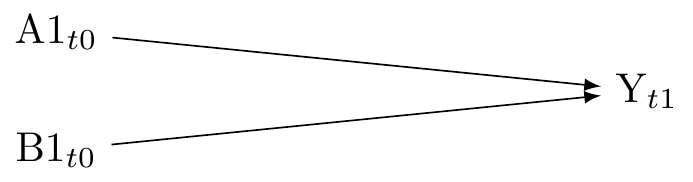
\includegraphics[width=0.4\textwidth,height=\textheight]{causal-dags_files/figure-pdf/fig-dag-interaction-1.pdf}

}

\caption{\label{fig-dag-interaction}Causal interaction: if two exposures
are causally independent of each other, we may wish to estimate their
individual and joint effects on Y, where the counterfactual outcome is
Y(a,b) and there is evidence for additive or subadditive interaction if
E{[}Y(1,1) - Y(0,1) - Y(1,0) + Y(0,0){]} ≠ 0. If we cannot conceptualise
B as a variable upon which there can be intervention, then the
interaction is better conceived as effect modification (see next
figure). Important: Causal diagrams are not parametric: do not attempt
to draw a path into another path.}

\end{figure}

\hypertarget{understanding-effect-modification-visualisation-on-graphs}{%
\subsubsection{\texorpdfstring{\textbf{Understanding Effect
Modification: Visualisation on
Graphs}}{Understanding Effect Modification: Visualisation on Graphs}}\label{understanding-effect-modification-visualisation-on-graphs}}

In the context of effect modification, we aim to understand how an
exposure's influence on an outcome fluctuates across different levels of
another variable. For instance, suppose we are investigating how the
impact of belief in Big Gods on social complexity varies across early
urban civilizations in China and South America. Here, ``geography''
(China versus South America) acts as an ``effect modifier.'' That is,
our research interest is in how the impact of our exposure (belief in
Big Gods) on the outcome (social complexity) shifts across various
``geography'' levels. It is vital to note that we are not treating the
effect modifier as an intervention variable, but merely as one that may
alter our exposure's effect on the outcome.

For clarity, consider a comparison between two exposure levels,
represented as \(A = a\) and \(A= a^*\). Further, assume that \(G\)
represents two levels of effect-modification, represented as \(g\) and
\(g'\). Then:

\[\hat{E}[Y(a)|G=g]\]

represents the expected outcome when exposure is at level \(A=a\) among
individuals in group \(G=g\).

\[\hat{E}[Y(a^*)|G=g]\]

represents the expected outcome when exposure is at level \(A=a^*\)
among individuals in group \(G=g\).

The difference

\[\hat{\delta}_g = \hat{E}[Y(a)|G=g] - \hat{E}[Y(a^*)|G=g]\]

estimates the causal effect of shifting the exposure from \(a^*\) to
\(a\) in group \(g\).

Similarly,
\[\hat{\delta}_{g'} = \hat{E}[Y(a)|G=g'] - \hat{E}[Y(a^*)|G=g']\]
estimates the causal effect of changing the exposure from \(a^*\) to
\(a\) in group \(g'\).

Comparing the causal effects between these two groups is achieved by
computing

\[\hat{\gamma} = \hat{\delta}_g - \hat{\delta}_{g'}\]

The value of \(\hat{\gamma}\) quantifies how the effect of shifting the
exposure from \(a^*\) to \(a\) differs between groups \(g\) and \(g'\).
If \(\hat{\gamma}\neq 0\), it implies the exposure's effect varies
between the two groups, indicating effect modification.

Again, it is vital to remember that these diagrams are non-parametric.
Hence, to represent effect modification, do not draw an intersecting
path or attempt other visualisations. Instead, draw two edges into the
exposure, as depicted in \textbf{?@fig-dag-effect-modification}. Always
remember that the primary goal of creating a causal graph is to evaluate
confounding and address the identification problem. Causal graphs do not
need to be parametric to do that work. Do not attempt to use them to do
other work. Again, ensuring the chronological order of events in your
graph's spatial layout will make the identification problem more
transparent since causes must precede effects.\footnote{For important
  distinctions within effect modification, see
  (\protect\hyperlink{ref-vanderweele2007}{\textbf{vanderweele2007?}}).}

\begin{figure}

{\centering 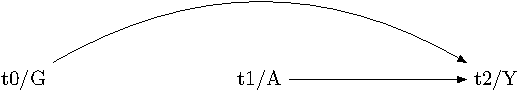
\includegraphics[width=0.8\textwidth,height=\textheight]{causal-dags_files/figure-pdf/fig-dag-effect-modfication-1.pdf}

}

\caption{\label{fig-dag-effect-modfication}A simple graph for
effect-modification.}

\end{figure}

\hypertarget{case-2-causal-mediation-causal-graphs-show-the-inadequacy-of-standard-approaches}{%
\subsection{Case 2: Causal mediation: causal graphs show the inadequacy
of standard
approaches}\label{case-2-causal-mediation-causal-graphs-show-the-inadequacy-of-standard-approaches}}

The conditions necessary for causal mediation are stringent.
Chronologically arranged causal diagrams, as shown in
Figure~\ref{fig-dag-mediation-assumptions}, can aid us in identifying
both the promise and perils of causal mediation. We will again keep to
the question of whether cultural beliefs in Big Gods affect social
complexity, and ask whether this affect is mediated by political
authority.

\begin{enumerate}
\def\labelenumi{\arabic{enumi}.}
\tightlist
\item
  \textbf{No unmeasured exposure-outcome confounders given} \(L\)
\end{enumerate}

This prerequisite is expressed as \(Y(a,m) \coprod A | L1\). Upon
controlling for the covariate set \(L1\), we must ensure that there are
no additional unmeasured confounders affecting both the cultural beliefs
in Big Gods \(A\) and the social complexity \(Y\). For example, if our
study involves the impact of cultural beliefs in Big Gods (exposure) on
social complexity (outcome), and geographic location and historical
context are our covariates \(L1\), this assumption of no unmeasured
confounding suggests that accounting for \(L1\) sufficiently covers any
subsequent correlation between \(A\) and \(Y\). The relevant confounding
path is depicted in brown in Figure~\ref{fig-dag-mediation-assumptions}.

\begin{enumerate}
\def\labelenumi{\arabic{enumi}.}
\setcounter{enumi}{1}
\tightlist
\item
  \textbf{No unmeasured mediator-outcome confounders given} \(L\)
\end{enumerate}

This condition is expressed as \(Y(a,m) \coprod M | L2\). Upon
controlling for the covariate set \(L2\), we must ensure that no other
unmeasured confounders affect both the political authority \(M\) and
social complexity \(Y\). For instance, if trade networks impact both
political authority and social complexity, we must account for trade
networks to obstruct the otherwise unblocked path linking our mediator
and outcome. Further, we must assume the absence of any other
confounders for the mediator-outcome path. This confounding path is
represented in blue in Figure~\ref{fig-dag-mediation-assumptions}.

\begin{enumerate}
\def\labelenumi{\arabic{enumi}.}
\setcounter{enumi}{2}
\tightlist
\item
  \textbf{No unmeasured exposure-mediator confounders given} \(L\)
\end{enumerate}

This requirement is represented as \(M(a) \coprod A | L3\). Upon
controlling for the covariate set \(L3\), we must ensure that there are
no additional unmeasured confounders affecting both the cultural beliefs
in Big Gods \(A\) and political authority \(M\). For example, the
capability to construct large ritual theaters may influence both the
belief in Big Gods and the level of political authority. If we have
indicators for this technology measured prior to the emergence of Big
Gods (these indicators being \(L3\)), we must assume that accounting for
\(L3\) is enough to obstruct the backdoor path between the exposure and
the mediator for unbiased natural mediated effect estimation. This
confounding path is shown in green in
Figure~\ref{fig-dag-mediation-assumptions}.

\begin{enumerate}
\def\labelenumi{\arabic{enumi}.}
\setcounter{enumi}{3}
\tightlist
\item
  \textbf{No mediator-outcome confounder affected by the exposure (no
  red arrow)}
\end{enumerate}

This requirement is indicated as \(Y(a,m) \coprod M^{a^*} | L\). We must
ensure that no variables confounding the relationship between political
authority and social complexity in \(L2\) are themselves influenced by
the cultural beliefs in Big Gods (\(A\)). For instance, when studying
the effect of cultural beliefs in Big Gods (\(A\), the exposure) on
social complexity (\(Y\), the outcome) mediated by political authority
(mediator), this assumption means that there are no factors, such as
trade networks (\(L2\)), that influence both political authority and
social complexity and are affected by the belief in Big Gods. This
confounding path is shown in red in
Figure~\ref{fig-dag-mediation-assumptions}. It is important to note that
\textbf{the assumption of no mediator/outcome confounder affected by the
exposure is challenging to satisfy}. If the exposure influences a
confounder of the mediator and outcome, we face a dilemma. If we do not
account for this confounder, the backdoor path between the mediator and
outcome remains open. By accounting for it, however, we partially
obstruct the path between the exposure and mediator, leading to bias.
Consequently, the natural direct and indirect effects can't be
identified from the manifest data, even with perfect measures of the
relevant confounders. Notice again that the requirements for
counterfactual data science are more strict than for descriptive or
predictive data science. Nonetheless, we can set the mediator to certain
levels and explore controlled direct and indirect effects, which may be
relevant for science and policy. For instance, if we were to fix
political authority at a specific level, we could ask, what would be the
direct and indirect causal effects of Big Gods on social complexity?
There are other approaches that involve sampling from the observed
distributions to obtain probablistic identification (an excellent
resource is (\protect\hyperlink{ref-shi2021}{\textbf{shi2021?}}) ).
Answering such questions typically necessitates the use of G-methods,
which the subsequent section will elaborate on. For now, we have seen
how chronologically ordered causal diagrams elucidate the conditions
necessary for mediation analysis in addressing causal
questions.\footnote{An excellent resource both for understanding causal
  interaction and causal mediation is
  (\protect\hyperlink{ref-vanderweele2015a}{\textbf{vanderweele2015a?}}).}

\begin{figure}

{\centering \includegraphics[width=0.8\textwidth,height=\textheight]{causal-dags_files/figure-pdf/fig-dag-mediation-assumptions-1.pdf}

}

\caption{\label{fig-dag-mediation-assumptions}Assumptions for mediation
analysis. The brown edges denote the path for common causes of the
exposure and coutcome. To block this path we must condition on L1. The
green edges denote the path for common causes of the exposure and
mediator. To block this path we must condition on L3. The blue edges
denote the path for common causes of the mediator and outcome. To block
this path we must condition on L2. The red path denotes the effect of
the exposure on the confounder of the mediator and outcome. If any such
path exists then we cannot obtain natural direct and indirect effects.
Conditioning on L2 is necessary to prevent mediator outcome confounding
but doing so blocks the effect of the exposure on the mediator.}

\end{figure}

\hypertarget{case-3-confounder-treatment-feedback-causal-graphs-show-the-inadequacy-of-standard-approaches}{%
\subsection{Case 3: Confounder-treatment feedback: causal graphs show
the inadequacy of standard
approaches}\label{case-3-confounder-treatment-feedback-causal-graphs-show-the-inadequacy-of-standard-approaches}}

Causal mediation is a special case in which we have multiple sequential
exposures. Here again chronologically organised causal diagrams can help
us to understand the problems and opportunities for causal inference
using time-series data.

For example, consider temporally fixed multiple exposures. The
counterfactual outcomes may be denoted \(Y(a_{t1} ,a_{t2})\). There are
four counterfactual outcomes corresponding to the four fixed ``treatment
regimes'':

\begin{enumerate}
\def\labelenumi{\arabic{enumi}.}
\item
  \textbf{Always treat (Y(1,1))}: This regime involves providing the
  treatment at every opportunity.
\item
  \textbf{Never treat (Y(0,0))}: This regime involves abstaining from
  providing the treatment at any opportunity.
\item
  \textbf{Treat once first (Y(1,0))}: This regime involves providing the
  treatment only at the first opportunity and not at subsequent one.
\item
  \textbf{Treat once second (Y(0,1))}: This regime involves abstaining
  from providing the treatment at the first opportunity, but then
  providing it at the second one.
\end{enumerate}

There are six causal contrasts that we might compute for the four fixed
regimes, presented in \textbf{?@tbl-regimes} \footnote{We compute the
  number of possible combinations of contrasts by
  \(C(n, r) = \frac{n!}{(n-r)! \cdot r!}\)}

\begin{longtable}[]{@{}
  >{\raggedright\arraybackslash}p{(\columnwidth - 4\tabcolsep) * \real{0.1351}}
  >{\raggedright\arraybackslash}p{(\columnwidth - 4\tabcolsep) * \real{0.5405}}
  >{\raggedright\arraybackslash}p{(\columnwidth - 4\tabcolsep) * \real{0.3243}}@{}}
\caption{Table describes four fixed treatment regimes and six causal
contrasts in time series data where the exposure may
vary.}\tabularnewline
\toprule\noalign{}
\begin{minipage}[b]{\linewidth}\raggedright
Type
\end{minipage} & \begin{minipage}[b]{\linewidth}\raggedright
Description
\end{minipage} & \begin{minipage}[b]{\linewidth}\raggedright
Counterfactual Outcome
\end{minipage} \\
\midrule\noalign{}
\endfirsthead
\toprule\noalign{}
\begin{minipage}[b]{\linewidth}\raggedright
Type
\end{minipage} & \begin{minipage}[b]{\linewidth}\raggedright
Description
\end{minipage} & \begin{minipage}[b]{\linewidth}\raggedright
Counterfactual Outcome
\end{minipage} \\
\midrule\noalign{}
\endhead
\bottomrule\noalign{}
\endlastfoot
Regime & Always treat & Y(1,1) \\
Regime & Never treat & Y(0,0) \\
Regime & Treat once first & Y(1,0) \\
Regime & Treat once second & Y(0,1) \\
Contrast & Always treat vs.~Never treat & E{[}Y(1,1) - Y(0,0){]} \\
Contrast & Always treat vs.~Treat once first & E{[}Y(1,1) - Y(1,0){]} \\
Contrast & Always treat vs.~Treat once second & E{[}Y(1,1) -
Y(0,1){]} \\
Contrast & Never treat vs.~Treat once first & E{[}Y(0,0) - Y(1,0){]} \\
Contrast & Never treat vs.~Treat once second & E{[}Y(0,0) - Y(0,1){]} \\
Contrast & Treat once first vs.~Treat once second & E{[}Y(1,0) -
Y(0,1){]} \\
\end{longtable}

Treatment could also be a function of the previous outcome. For example,
we might \textbf{Treat once first} and then decide to treat again or not
treat again depending on the outcome of the initial treatment. This is
known as ``time-varying treatment regimes.''

It is important to remember that to estimate the ``effect'' of a
treatment regime, we must compare the counterfactual quantities of
interest. The same conditions that apply for causal identification in
mediation analysis also apply to causal identification in multiple
treatment settings. Just as mediation introduces the possibility of
time-varying confounding (condition 4, where the exposure affects the
confounders of the mediator/outcome path), so too we discover that
time-varying treatments introduce the issue of time-varying confounding.
Unlike traditional causal mediation analysis, the sequence of treatment
regimes we might consider can be indefinitely long.

Chronologically organised causal diagrams are again instrumental in
highlighting the issues with traditional multi-level regression analysis
and structural equation modelling. For example, we may be interested in
whether belief in Big Gods affects social complexity.

Consider fixed regimes first. If we have a well-defined concept of
social complexity and excellent measurements over time, we might want to
compare the effects of beliefs in Big Gods on social complexity using
historical data gathered over two centuries. Our query is whether the
introduction and persistence of such beliefs are different from having
no such beliefs. The treatment strategies are: ``always believe in Big
Gods'' versus ``never believe in Big Gods'' on the level of social
complexity. Refer to Figure~\ref{fig-dag-9}. Here, \(A_{tx}\) represents
the cultural belief in Big Gods at time \(tx\), and \(Y_{tx}\) is the
outcome, social complexity, at time \(x\). Economic trade, denoted as
\(L_{tx}\), is a time-varying confounder because it changes over time
and confounds the effect of \(A\) on \(Y\) at several time points \(x\).
To complete our causal diagram, we include an unmeasured confounder
\(U\), such as oral traditions, which might influence both the belief in
Big Gods and social complexity.

We know that the level of economic trade at time \(0\), \(L_{t0}\),
influences the belief in ``Big Gods'' at time \(1\), \(A_{t1}\). We
therefore draw an arrow from \(L_{t0}\) to \(A_{t1}\). But we also know
that the belief in ``Big Gods'', \(A_{t1}\), affects the future level of
economic trade, \(L_{t(2)}\). This means that we need to add an arrow
from \(A_{t1}\) to \(L_{t2}\). This causal graph represents a feedback
process between the time-varying exposure \(A\) and the time-varying
confounder \(L\). This is the simplest graph with exposure-confounder
feedback. In real world setting there would be more arrows. However, our
DAG need only show the minimum number of arrows to exhibit the problem
of exposure-confounder feedback. (We should not clutter our causal
diagrams: only provide the essential details.)

What happens if we were to condition on the time-varying confounder
\(L_{t3}\)? Two things would occur. First, we would block all the
backdoor paths between the exposure \(A_{t2}\) and the outcome. We need
to block those paths to eliminate confounding. Therefore, conditioning
on the time-varying confounding is essential. However, paths that were
previously blocked would not be pen. For example, the path
\(A_{t1}, L_{t2}, U, Y_{t(4)}\), which was previous closed is opened
because the time varying confounder is the common effect of \(A_{t1}\)
and \(U\). Conditioning opens the path \(A_{t1}, L_{t2}, U, Y_{3}\).
Therefore we must avoid conditioning on the time varying confounder. We
are damned-if-we-do-or-do-not condition on the confounder that is
affected by the prior exposure.

\begin{figure}

{\centering 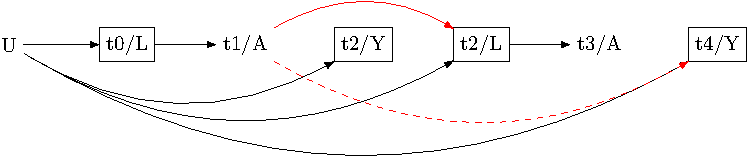
\includegraphics[width=1\textwidth,height=\textheight]{causal-dags_files/figure-pdf/fig-dag-9-1.pdf}

}

\caption{\label{fig-dag-9}Exposure confounder feedback is a problem for
time-series models. If we do not condition on L\_t2, a backdoor path is
open from A\_t3 to Y\_t4. However, if conditioning on L\_t2 introduces
collider bias, opening a path, coloured in red, between A\_t2 and Y\_t4.
Here, we may not use conventional methods to estimate the effects of
multiple exposures. Instead, at best, we may only simulate controlled
effects using G-methods. Multi-level models will eliminate bias.
Currently, outside of epidemiology, G-methods are rarely used. causal
diagrams are useful for clarifying the damned either way confounding
control strategies that lead traditional methods to fail.}

\end{figure}

A similar problem arises when the time-varying exposure and time-varying
confounder share a common cause. The problem arises even without the
exposure affecting the confounder, as presented in
Figure~\ref{fig-dag-time-vary-common-cause-A1-l1}.

\begin{figure}

{\centering 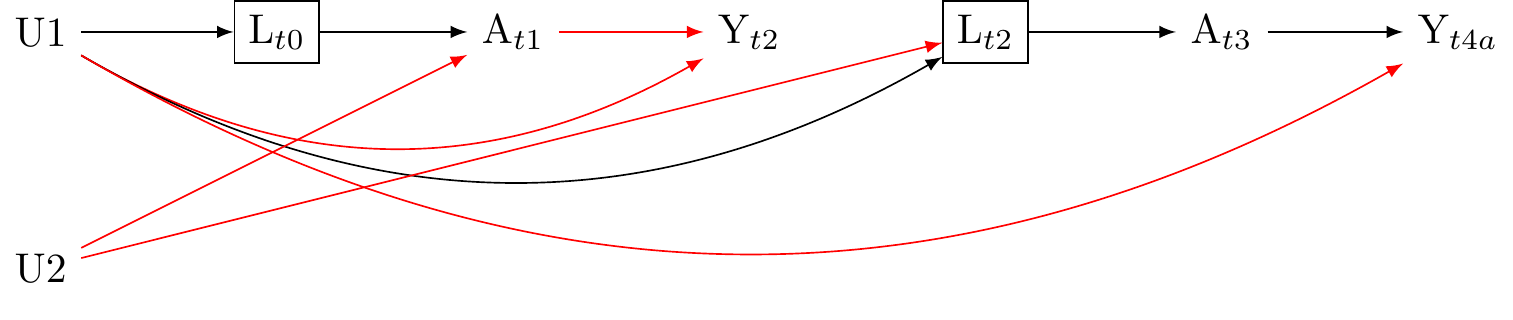
\includegraphics[width=1\textwidth,height=\textheight]{causal-dags_files/figure-pdf/fig-dag-time-vary-common-cause-A1-l1-1.pdf}

}

\caption{\label{fig-dag-time-vary-common-cause-A1-l1}Exposure confounder
feedback is a problem for time-series models. Here, the problem arises
from an unmeasured variable (U2) that affects both the exposure A at
time 1 and the counfounder L at time 2. The red paths show the back door
path that is opened when we condition on the L at time 2. Again, this
problem cannot be addressed with regression-based methods. In this
setting, to address causal questions, we may only use simulation based
G-methods. causal diagrams are useful in clarifying problems for
identifying causal effects from manifest data, even when the data are
large and perfectly measured.}

\end{figure}

The complexity grows when the exposure \(A_{t1}\) influences the outcome
\(Y_{t4}\). For instance, because \(L_{t2}\) lies on the pathway from
\(A_{t1}\) to \(Y_{t4}\), conditioning on \(L_{t2}\) partially obstructs
the connection between exposure and outcome. Such conditioning triggers
both collider stratification bias and mediator bias. However, to close
the open backdoor path between \(L_{t2}\) and \(Y_{t4}\), conditioning
on \(L_{t2}\) is necessary, yet it is also necessary not to do so to
avoid mediation bias. The broader challenge of exposure-confounder
feedback is detailed in
(\protect\hyperlink{ref-hernan2023b}{\textbf{hernan2023b?}}). This issue
poses a significant problem for cultural evolutionary studies, as
conventional regression-based methods --- including multi-level
regression --- are incapable of solving identification issues amidst
time-varying confounding (\protect\hyperlink{ref-robins}{J. M. Robins
and Hernán, n.d.}; \protect\hyperlink{ref-robins1986}{J. Robins 1986}).

Models suited for evaluating the causal effects of time-fixed and
time-varying exposures are encompassed by ``G-methods''
(\protect\hyperlink{ref-naimi2017}{\textbf{naimi2017?}};
\protect\hyperlink{ref-chatton2020}{\textbf{chatton2020?}};
\protect\hyperlink{ref-robins}{J. M. Robins and Hernán, n.d.};
\protect\hyperlink{ref-hernuxe1n2006}{\textbf{hernán2006?}}). Even
though these methods have seen considerable development recently in the
health sciences
(\protect\hyperlink{ref-williams2021}{\textbf{williams2021?}};
\protect\hyperlink{ref-duxedaz2021}{\textbf{díaz2021?}};
\protect\hyperlink{ref-breskin2021}{\textbf{breskin2021?}}), their
adoption in cultural evolutionary research is still fledgling. The
efficacy of causal diagrams permeates longitudinal research, including
cultural evolution, underscoring that traditional methods like
multi-level regression models are generally ineffective at precisely
identifying causal effects from time-series data with
treatment-confounder feedback\footnote{It is worth noting that the
  identification of controlled effect estimates can benefit from
  graphical methods such as ``Single World Intervention Graphs''
  (SWIGs), which depict counterfactual outcomes. Nevertheless, SWIGs in
  their general form are templates rather than causal diagrams and their
  application extends beyond this tutorial's scope. Refer to
  (\protect\hyperlink{ref-richardson2013}{\textbf{richardson2013?}}) for
  more on SWIGs.}.

\hypertarget{summary-part-2}{%
\subsection{Summary Part 2}\label{summary-part-2}}

To estimate causal effects we must contrast the world as it has been
with the world as it might have been. For many questions in cultural
evolution, we have seen confounder-treatment feedback leads to
intractable identification problems. We have also seen that causal
diagrams are useful for clarifying these problems. Throughout we have
seen the advantages of chronologically order in our graphs. With the
exception of proxy variables, many self-inflicted injuries such as
mediator bias, and post-stratification bias can be avoided when
confounders are measured prior to the exposures. Chronologically ordered
causal graphs aim to make this basis transparent.

I next turn to three-wave designs for estimating the total causal
effects. Such designs have applications for a broad class of cultural
evolutionary questions, and may be especially useful for evolutionary
anthropologists who wish to collect time-series data in the present to
address causal questions about cultural evolution as it is occurring in
the world today.

\hypertarget{part-3.-applications-the-three-wave-panel-design.}{%
\section{Part 3. Applications: the three wave panel
design.}\label{part-3.-applications-the-three-wave-panel-design.}}

In this section, we explore how temporally ordered causal diagrams can
illuminate the utility of a three-wave panel design for addressing
causal questions using data.

\hypertarget{step-1.-specify-the-exposure-and-measure-it-at-wave-0-and-wave-1.}{%
\subsection{Step 1. Specify the exposure and measure it at wave 0 and
wave
1.}\label{step-1.-specify-the-exposure-and-measure-it-at-wave-0-and-wave-1.}}

Initially, we need a well-defined exposure. Unless our interest is in
causal interaction, causal mediation, or sequential treatment regimes,
we will investigate the total effect of only one exposure. Suppose we
are interested in investigating the causal effect of religious service
attendance. Our first task is to explicitly state the the exposure as a
hypothetical intervention: Is our interest in any attendance versus
non-attendance?, weekly attendance versus monthly attendance? or some
other state. Imagining a hypothetical experiment, even if not feasible,
helps to focus on the need to state a clear intervention
(\protect\hyperlink{ref-hernuxe1n2022a}{\textbf{hernán2022a?}}).

In a three-wave panel design, we must measure the exposure both at
baseline and at the second wave. This dual measurement strategy plays a
crucial role in the effort to use observational data to replicate the
design of a controlled experiment. When an exposure is recorded at the
baseline and the second wave, we ensure that what we are assessing is
the effect of the ``incident exposure'' - an exposure newly occurring
between the first and second waves. This is distinct from the
``prevalent exposure,'' that is the frequency of the distribution of
exposure in the population at baseline
(\protect\hyperlink{ref-danaei2012}{\textbf{danaei2012?}};
\protect\hyperlink{ref-hernan2023}{\textbf{hernan2023?}}). By
controlling for baseline exposure we more effectively emulate an
experimental manipulation of a factor of interest, wherein an
intervention is applied at a particular point in time and subsequent
changes are observed. Consider how biase might occur if the exposure is
initially harmful to the outcome. Suppose we only measure the exposure
at the second wave and ignore the initial exposure at baseline (see:
Figure~\ref{fig-dag-descendent-solution-2}.). In that case, we might
wrongly infer that the exposure is benefitial
(\protect\hyperlink{ref-hernuxe1n2008a}{\textbf{hernán2008a?}};
\protect\hyperlink{ref-hernuxe1n2016a}{\textbf{hernán2016a?}}).

An further advantage of controlling for the exposure at baseline is that
it can reduce the probability of bias that might arise if there is an
unmeasured confounder affecting both the outcome and the initial
exposure, irrespective of the previous exposure levels.

\hypertarget{caution-if-the-exposure-is-rare-large-amounts-of-data-must-be-collected-to-estimate-causal-effects}{%
\subsubsection{\texorpdfstring{\textbf{Caution: if the exposure is rare,
large amounts of data must be collected to estimate causal
effects}}{Caution: if the exposure is rare, large amounts of data must be collected to estimate causal effects}}\label{caution-if-the-exposure-is-rare-large-amounts-of-data-must-be-collected-to-estimate-causal-effects}}

\hypertarget{part-3.-applications-the-three-wave-panel-design}{%
\section{Part 3. Applications: The Three-Wave Panel
Design}\label{part-3.-applications-the-three-wave-panel-design}}

In this section, we discuss how temporally ordered causal diagrams can
help illustrate the benefits of a three-wave panel design in addressing
causal queries using data.

\hypertarget{step-1.-defining-the-exposure-and-its-measurement-at-wave-0-and-wave-1}{%
\subsection{Step 1. Defining the Exposure and Its Measurement at Wave 0
and Wave
1}\label{step-1.-defining-the-exposure-and-its-measurement-at-wave-0-and-wave-1}}

We start with a well-defined exposure. Unless our focus lies in causal
interaction, causal mediation, or sequential treatment plans, our task
will be to examine the total effect of a single exposure.

Consider the causal effect of attending religious services. Our primary
task is to define the exposure as a hypothetical intervention. What
interests us: any attendance versus non-attendance? Weekly attendance
versus monthly attendance? Or something else? Imagining a hypothetical
experiment, even if impractical, highlights the importance of specifying
a clear intervention
(\protect\hyperlink{ref-hernuxe1n2022a}{\textbf{hernán2022a?}}).

In a three-wave panel design, we must capture the exposure at both the
baseline and second wave. This two-fold measurement approach is crucial
for using observational data to simulate a controlled experiment. By
recording the exposure at the baseline and second wave, we ensure that
we measure the effect of the ``incident exposure'' - an exposure newly
appearing between the first and second waves. This differs from the
``prevalent exposure,'' which is the baseline distribution of exposure
in the population
(\protect\hyperlink{ref-danaei2012}{\textbf{danaei2012?}};
\protect\hyperlink{ref-hernan2023}{\textbf{hernan2023?}}). Controlling
for baseline exposure helps us emulate an experimental manipulation more
effectively, wherein we apply an intervention at a particular moment and
observe the ensuing changes. Consider potential biases if the initial
exposure harms the outcome. If we measure the exposure only at the
second wave and overlook the baseline exposure, we might incorrectly
conclude that the exposure is beneficial
(\protect\hyperlink{ref-hernuxe1n2008a}{\textbf{hernán2008a?}};
\protect\hyperlink{ref-hernuxe1n2016a}{\textbf{hernán2016a?}}).

Controlling for exposure at the baseline also has an additional benefit:
it can lower the probability of bias that may occur if an unmeasured
confounder affects both the outcome and the initial exposure,
irrespective of previous exposure levels.

\hypertarget{note-large-data-quantities-must-be-collected-to-estimate-causal-effects-if-the-exposure-is-rare}{%
\subsubsection{\texorpdfstring{\textbf{Note: Large data quantities must
be collected to estimate causal effects if the exposure is
rare}}{Note: Large data quantities must be collected to estimate causal effects if the exposure is rare}}\label{note-large-data-quantities-must-be-collected-to-estimate-causal-effects-if-the-exposure-is-rare}}

Assume in the non-religious population the switch from no religious
service attendance to weekly attendance is rare, say 1 in 1,000
non-attenders per year. Acquiring an effective sample for a
``treatment'' group, while conditioning on a rich set of variables,
might not be feasible without hundreds of thousands of participants. It
might be more practical to consider changes within the religious
population, assuming changes are more common within this group. However,
we would then typically estimate a causal effect that generalises to the
religious population from which the sample was drawn, rather than one
that transports to the non-religious population.

\hypertarget{step-2.-defining-the-outcomes-and-their-measurement-at-wave-0-and-wave-2}{%
\subsection{Step 2. Defining the Outcome(s) and Their Measurement at
Wave 0 and Wave
2}\label{step-2.-defining-the-outcomes-and-their-measurement-at-wave-0-and-wave-2}}

After defining the exposure, we need to specify a well-defined outcome,
or multiple outcomes. For instance, we might be interested in how
gaining or losing religious beliefs affects the frequency of
volunteering (e.g., weekly, monthly, yearly). Vague concepts such as
``the causal effects of religious change'' don't lead us to understand
causality. We must specify what we mean by ``religious change'' by
identifying an intervention and ``societal effect'' by defining a
measurable outcome that occurs post-intervention.

In a three-wave panel design, outcomes are recorded at the baseline (for
confounding control) and the third wave, which follows the exposure.
Although we are generally limited to estimating the effect of a single
exposure at a time, we aren not confined to estimating the effects of
exposure on just one outcome. Indeed, we advance understanding more
rapidly by evaluating a spectrum of responses across as many exposures
as are relevant to the area of interest
(\protect\hyperlink{ref-vanderweele2020}{\textbf{vanderweele2020?}}).

In a three-wave panel design, outcomes need to be recorded at the
baseline (for confounding control) and two waves from the baseline. It
is crucial to control for the outcome measured at the baseline -- the
`baseline outcome' -- to verify the correct temporal order of the
cause-effect relationship, i.e., to prevent reverse causation. Moreover,
when the exposure is also controlled for at the baseline, then for an
unmeasured confounder to explain away the association between the
exposure one wave from the baseline and the outcome two waves from the
baseline, it would need to do so independently of the baseline effect.
This scenario is depicted in Figure~\ref{fig-dag-6}. This causal diagram
makes an essential practical point: although confounding might not be
entirely eliminated (the dashed arrows symbolise the potential for
uncontrolled sources of bias), data collection and analysis can reduce
bias. Given we can almost never be sure we have controlled for
unmeasured confounding, researchers should perform sensitivity analyses
(another important topic that we unfortuantely do not have space to
explore here).

\begin{figure}

{\centering 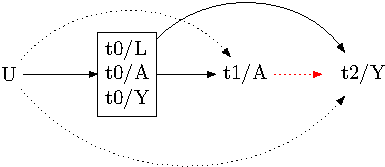
\includegraphics[width=0.8\textwidth,height=\textheight]{causal-dags_files/figure-pdf/fig-dag-6-1.pdf}

}

\caption{\label{fig-dag-6}Causal graph: adapted from Vanderweele et al's
three-wave panel design. The blue-dotted line indicates a reduction in
bias arising from the strategy of including baseline measures for the
exposure and outcome. For an unmeasured confounder U to bias the
exposure outcome association it would need to do so independently of
these baseline measures of the outcome and exposure. The graph
furthermore clarifies that by measuring confounders before the exposure
and the exposure before the outcome, we reduce the potential for reverse
causation, collider stratification, and mediator biases.}

\end{figure}

\hypertarget{step-3.-identify-observable-common-causes-of-the-exposure-and-the-outcome-and-group-them-under-simplified-labels}{%
\subsection{Step 3. Identify observable common causes of the exposure
and the outcome, and group them under simplified
labels}\label{step-3.-identify-observable-common-causes-of-the-exposure-and-the-outcome-and-group-them-under-simplified-labels}}

Next, we should identify all the potential confounders that, when
adjusted for, can eliminate any non-causal association between the
exposure and outcome. We should group these confounders under labels
where possible. In a three-wave panel design, these confounders are
typically recorded during the baseline wave, preceding the exposure. As
illustrated in Figure~\ref{fig-dag-mediator-solution}, recording
confounders before exposure minimises the potential for mediation bias.

\hypertarget{step-4.-gather-data-for-proxy-variables-of-unmeasured-common-causes-at-the-baseline-wave}{%
\subsection{Step 4. Gather data for proxy variables of unmeasured common
causes at the baseline
wave}\label{step-4.-gather-data-for-proxy-variables-of-unmeasured-common-causes-at-the-baseline-wave}}

If there exist any unmeasured factors influencing both the exposure and
outcome, but we lack direct measurements for them, efforts should be
made to include proxies for these factors, as outlined in
Figure~\ref{fig-dag-descendent-solution-2}. Again, even if this strategy
cannot be ensured to eliminate bias, it may reduce bias from unmeasured
confounding.

\hypertarget{step-5.-state-the-target-population-for-whom-the-causal-question-applies}{%
\subsection{Step 5. State the target population for whom the causal
question
applies}\label{step-5.-state-the-target-population-for-whom-the-causal-question-applies}}

We need to define for whom our causal inference applies. For this
purpose, it is useful to distinguish the concepts of source population
and target population, and between the concepts of generalisability and
transportability.

\begin{enumerate}
\def\labelenumi{\arabic{enumi}.}
\item
  \textbf{The source population} is the population from whom our sample
  is drawn.
\item
  \textbf{The target population} is the larger group for which we aim to
  apply our study's results. The closer the source matches the target in
  ways that are relevant to our causal questions, the stronger our
  causal inferences about the target population will be.
\item
  \textbf{Generalisability} refers to the ability to apply the causal
  effects estimated from a sample to the source population. Researchers
  in the human sciences know this concept as ``external validity.''
  Where:
\end{enumerate}

\begin{enumerate}
\def\labelenumi{\alph{enumi}.}
\tightlist
\item
  \(PATE\) denotes the population average treatment effect for the
  target population.
\item
  \(ATE_{\text{source}}\) denotes the average treatment effect in the
  source population.
\item
  \(W\) denotes a set of variables upon which the source and target
  population might differ when the research interest is in transporting
  resultes to a population other than that from which the source
  population is drawn.
\item
  \(T\) denotes a set of variables upon which the source and the target
  population might differ when the interest is in generalising beyond
  the population from which the source population is drawn.
\end{enumerate}

We may define \emph{generalisability} such that:

\[PATE =  f(ATE_{\text{source}}, W)\]

Results generalise if the population average treatment effect in the
target population can be expressed as a function of the average
treatment effect in the source population and the set of variables,
\(W\), which differentiate the two populations. This function is a
mapping of the average treatment effect from the source population,
adjusted for the observed differences between the populations,
represented by \(W\). Here, \(f\) could be a model or a set of
transformations capturing the relationship between the source and target
populations' treatment effects, conditioned on \(W\). It might involve
rescaling, weighting, or modelling interactions.

\begin{enumerate}
\def\labelenumi{\arabic{enumi}.}
\setcounter{enumi}{3}
\tightlist
\item
  \textbf{Transportability} refers to the ability to extrapolate causal
  effects learned from a source population to a target population. It
  pertains to the transfer of causal knowledge across different settings
  or populations such that
\end{enumerate}

\[ATE_{\text{target}} \approx f(ATE_{\text{source}}, T)\]

This function similarly maps the average treatment effect from the
source population to a target population. However, the target population
in this case differs from the population from which the source was
drawn. The structures that enable inference are denoted by \(T\). The
function over \(T\) might be more complex, as it must handle potential
heterogeneity of effects and unobserved sources of bias. To assess
transportability we generally require information about both the source
and target populations and an understanding of how the relationships
between treatment, outcome, and covariates might differ between the two
populations. Assessing transportability typically requires additional
data or specialist knowledge. In Section 4, we consider the concepts of
generalisability and transportability as they relate to sample
selection.

\hypertarget{step-6.-retention-is-critical}{%
\subsection{Step 6. Retention is
critical}\label{step-6.-retention-is-critical}}

For reasons we clarify in Part 4, retention of the original sample is
vital. Panel attrition not increases uncertainty by reducing the
effective sample size of a study at baseline, it opens novel pathways
for bias. Researchers must develop protocols for tracking individuals
over time as they change address, email, phone numbers, and names.
Moreover, developing and implementing strategies for motivating
retention of across the entire population of interest (not merely those
willing to volunteer for science) is critical for effective causal human
science. These strategies must be developed with specialist knowledge of
the population under study, and with the participation of people being
studied -- a topic for another article.

\hypertarget{summary-of-part-3}{%
\subsection{Summary of Part 3}\label{summary-of-part-3}}

The strengths of three-wave panel designs for confounding control is
demonstrated in Figure~\ref{fig-dag-6}. This diagram, adapted from
(\protect\hyperlink{ref-vanderweele2020}{\textbf{vanderweele2020?}}),
highlights the potential for residual unmeasured confounding even after
incorporating baseline measurements for both the exposure and outcome,
represented by the blue-dotted line. As such, for an unmeasured
confounder \(U\) to exert bias on the association between the exposure
\(A_{t1}\) and outcome \(Y_{t2}\), it must do so independently of the
baseline measurements of the exposure \(A_{t0}\) and outcome \(Y_{t0}\).

The diagram also clarifies the advantage of three-wave panel designs in
addressing reverse causation. This is achieved by controlling for both
the exposure and outcome at baseline, ensuring a robust temporal
sequence. Moreover, the diagram underscores the capacity of three-wave
panel designs to yield estimates of the incidence, not just prevalence,
of the effect.

Another crucial insight from Figure~\ref{fig-dag-6} pertains to the
potential pitfalls of collider stratification and mediator bias, both of
which arise when conditioning inadvertently occurs on a post-treatment
variable, as discussed in Part 2. By sequencing the measurement of
confounders prior to the exposure, and the exposure prior to the
outcome, we minimise these biases.

Figure~\ref{fig-dag-6} underscores their importance in directing the
collection of repeated measures data with specific attributes. However
(\protect\hyperlink{ref-vanderweele2020}{\textbf{vanderweele2020?}})'s
version leaves out the bias that might arise from panel attrition. In
part 4 we extend this graph to consider the threats that panel attrition
brings to causal inference.

\hypertarget{part-4.-exploring-selection-bias-in-the-three-wave-panel-design}{%
\subsection{Part 4. Exploring Selection Bias in the Three-Wave Panel
Design}\label{part-4.-exploring-selection-bias-in-the-three-wave-panel-design}}

\hypertarget{introduction-to-selection-bias}{%
\subsection{Introduction to Selection
Bias}\label{introduction-to-selection-bias}}

Selection bias may be broadly defined as the discrepancy between the
parameter of interest in a target population and the same parameter in a
subset of the population used for analysis - the source population
(\protect\hyperlink{ref-hernuxe1n2017}{\textbf{hernán2017?}}). This can
occur if the source population differs from the target population in
terms of descriptive parameters. In causal inference, our concern is how
selection bias might impact the estimation of causal effects. In other
words, how might differences between the source and target populations
influence causal contrasts on specific scales of interest (difference,
risk ratio, etc.). Causal diagrams help to clarify what is at stake.

However, before diving in, consider the following topology of
confounding according to Suzuki and colleagues
{[}(\protect\hyperlink{ref-suzuki2016}{\textbf{suzuki2016?}});
(\protect\hyperlink{ref-suzuki2014}{\textbf{suzuki2014?}}); Suzuki,
Shinozaki, and Yamamoto
(\protect\hyperlink{ref-suzuki2020}{2020}){]}\footnote{This typology
  builds on VanderWeele's work
  (\protect\hyperlink{ref-vanderweele2012}{\textbf{vanderweele2012?}}).}

\begin{enumerate}
\def\labelenumi{\arabic{enumi}.}
\item
  \textbf{Confounding in Distribution}: This term applies when the group
  exposed to each level of exposure is representative of the target
  population. In such cases, we say there is no confounding in the
  distribution of the exposure's effect on the outcome.
\item
  \textbf{Confounding in Expectation}: When the exposure assignment
  mechanism balances the confounders across each level of exposure to be
  contrasted, we say there is no confounding in the expectation of the
  exposure's effect on the outcome.
\item
  \textbf{Confounding in Measure}: If a specific measure of interest
  matches the corresponding causal measure in the target population, we
  say there is no confounding in the measure of the exposure's effect on
  the outcome. This is important because, as discussed previously in
  relation to interaction, our inference of a causal effect can depend
  on the scale of the causal effect measure.
\item
  \textbf{Realised Confounding}: If a specific exposure assignment leads
  to balance, irrespective of the exposure assignment mechanism, we say
  there is no realised confounding of the exposure's effect on the
  outcome. This is key, as even in randomised experiments, randomisation
  might not eliminate chance imbalances in the distributions of
  confounders across the exposures.
\end{enumerate}

Each of these four concepts plays a role in discussions of
``confounding,'' and all are crucial when evaluating a study's
scientific merit. However, each concept highlights different issues.

Armed with these distinctions, consider
Figure~\ref{fig-selection-under-the-null}, which presents a scenario
with no (marginal) causal effect of exposure on the outcome, yet a
degree of selection into the study. We will assume randomisation
succeeded and that are no arrows into \(A\). As
Figure~\ref{fig-selection-under-the-null} shows, neither confounding in
expectation nor in distribution is present. The null effect estimate
from the study will accurately reflect the true null effect in the
population. We might say that selection leads to ``confounding in
distribution for confounding in expectation.'' More simply, we can say
that despite selection, the null effect in the source population is not
biased for the target population, ensuring our null results generalise
(\protect\hyperlink{ref-hernuxe1n2004b}{\textbf{hernán2004b?}};
\protect\hyperlink{ref-greenlands.1977a}{\textbf{greenlands.1977a?}}).

\begin{figure}

{\centering 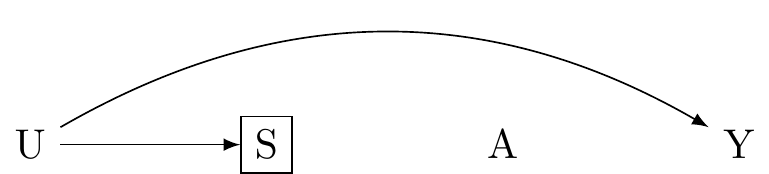
\includegraphics[width=0.6\textwidth,height=\textheight]{causal-dags_files/figure-pdf/fig-selection-under-the-null-1.pdf}

}

\caption{\label{fig-selection-under-the-null}Selection under the null.
An unmeasured variable affects selection into the study and the outcome.
D-separation is preserved there is no confounding in expectation.}

\end{figure}

Figure~\ref{fig-selection-off-the-null} presents a different scenario in
which there selection bias for the population parameter: the association
in the population of selected individuals differs from the causal
association in the target population. Hernán calls this scenario
``selection bias off the null''
(\protect\hyperlink{ref-hernuxe1n2017}{\textbf{hernán2017?}}). Lu et al
call this scenario ``type 2 selection bias''
(\protect\hyperlink{ref-lu2022a}{\textbf{lu2022a?}}). This bias occurs
because the selection into the study occurs on an effect modifier for
the effect of the exposure on the outcome. Note that although the causal
effect of \(A\to Y\) is unbiased for the exposed and unexposed in the
source population, the effect estimate does not generalise to the
exposed and unexposed in the target population:
\(PATE \cancel{\approx} ATE_{\text{sample}}\).

\begin{figure}

{\centering 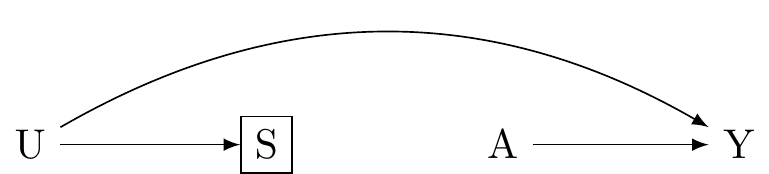
\includegraphics[width=0.6\textwidth,height=\textheight]{causal-dags_files/figure-pdf/fig-selection-off-the-null-1.pdf}

}

\caption{\label{fig-selection-off-the-null}Selection off the null: an
unmeasured variable affects selection into the study and the outcome.
Here the exposure affects the outcome. Although D-separation is
preserved, there there is confounding in distribution.}

\end{figure}

There has been considerable work investigating the conditions under
which causal estimates for a target population may be identified when
the source population differs from the target population, i.e.~whether
we may obtain a function such that \(PATE = f(ATE_{\text{source}}, W)\)
{[}see: (\protect\hyperlink{ref-lu2022a}{\textbf{lu2022a?}}){]}. There
has also been considerable recent work investigating whether results
transport to populations that systematically differ from the source
population -- i.e.~whether we may obtain a function such that
\(ATE_{\text{target}} \approx f(ATE_{\text{source}}, T)\) {[}see:
(\protect\hyperlink{ref-bareinboim2022a}{\textbf{bareinboim2022a?}};
\protect\hyperlink{ref-deffner2022a}{\textbf{deffner2022a?}}){]}. When
developing a three-wavel panel, to address type 2 selectiong bias we
must accurately measuring and properly adjust for a sufficient set of
covariates that affect selection \(\framebox{S}\) and the outcome in the
target population (\protect\hyperlink{ref-lu2022a}{\textbf{lu2022a?}}).
Moreover, when drawing a causal diagram, it is vital to present
confounding as it exists in the target population (see Suzuki,
Shinozaki, and Yamamoto (\protect\hyperlink{ref-suzuki2020}{2020})
especially their examples in the supplement.)

\hypertarget{selection-bias-in-which-both-the-exposure-and-outcome-affect-selection}{%
\subsection{Selection bias in which both the exposure and outcome affect
selection}\label{selection-bias-in-which-both-the-exposure-and-outcome-affect-selection}}

In panel designs there is additionally a constant threat of selection
occurring \emph{after} enrolment into the study. We next put
chronological causal diagrams to use in making sense of this threat, and
to derive practical advice.

We next use causal diagrams to clarify biases arising from panel
attrition. Panel attrition can be viewed as a special case of selection
bias because the participants who continue in a longitudinal study may
differ from those who drop out in ways that generate structural biases.

Figure~\ref{fig-dag-8-5}, describes a scenario in which both the
exposure and the true outcome affect panel attrition, biasing the
observed association between the exposure and the measured outcome in
the remaining sample. The problem of selection here is a problem
collider stratification bias. The problem can be equivalently viewed as
one of directed measurement error, described in the next section in
Figure~\ref{fig-dag-indep-d-effect}. Either way, restricting analysis to
the retained sample introduces bias in the the causal effect estimate by
opening a backdoor path from the exposure to the outcome.
(\protect\hyperlink{ref-lu2022a}{\textbf{lu2022a?}}) call this form of
bias: ``type 1 selection bias'' and distinguish between scenarios when
causal effects that generalise are recoverable (type 1a selection bias)
and not recoverable (type 1b selection bias). In both cases, we must
develop strategies to recover target population estimates from a subset
of the source population for which causal effect estimates may be biased
\textbf{for the source population.}

\begin{figure}

{\centering 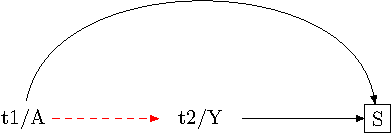
\includegraphics[width=0.8\textwidth,height=\textheight]{causal-dags_files/figure-pdf/fig-dag-8-5-1.pdf}

}

\caption{\label{fig-dag-8-5}Causal graph:outcome and exposure affect
attrition.}

\end{figure}

\hypertarget{unmeasured-confounder-affects-outcome-and-variable-that-affects-attrition}{%
\subsection{Unmeasured confounder affects outcome and variable that
affects
attrition}\label{unmeasured-confounder-affects-outcome-and-variable-that-affects-attrition}}

Figure Figure~\ref{fig-dag-8-2} presents another problem of selection
bias in a three-wave panel design. This diagram shows how an unmeasured
confounder, U\(_S\), can simultaneously influence the outcome variable
Y\(_{t2}\) and another variable, L\(_{t2}\), responsible for attrition
(i.e., the drop-out rate, denoted as \(\framebox{S}\)). In this
instance, the exposure variable, \(A_{t1}\), can impact L\(_{t2}\),
which subsequently affects attrition, \(\framebox{S}\). If the study's
selected sample descends from L\(_2\), the selection effectively
conditions on L\(_{t2}\), introducing potential bias into the analysis.
The diagram marks this possible biasing pathway with red-dashed lines.
Ordering the nodes chronologically elucidates the temporal sequence of
these events, allowing for a clearer assessment of potential bias
sources relevant to a three-wave panel design.

\begin{figure}

{\centering 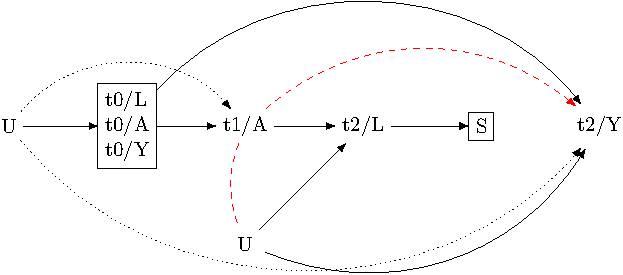
\includegraphics[width=0.8\textwidth,height=\textheight]{causal-dags_files/figure-pdf/fig-dag-8-2-1.pdf}

}

\caption{\label{fig-dag-8-2}Causal graph: three-wave panel design with
selection bias: example 2: Unmeasured confounder U\_S, is a cause of
both of the outcome Y\_2 and of a variable, L\_2 that affects attrition,
S. The exposure A affect this cause L\_2 of attrition, S. The selected
sample is a descendent of L\_2. Hence selection is a form of
conditioning on L\_2. Such conditioning opens a biasing path, indicated
by the red-dashed lines.}

\end{figure}

\hypertarget{summary-part-4-key-recommendations}{%
\subsection{Summary Part 4: Key
recommendations}\label{summary-part-4-key-recommendations}}

In this segment, we have leveraged causal diagrams to elucidate
potential confounding sources due to selection bias within the context
of longitudinal research. This process underscores the practical utility
of causal diagrams in research planning. Here are the essential
recommendations:

\begin{enumerate}
\def\labelenumi{\arabic{enumi}.}
\item
  \textbf{Broad Sampling}: To ensure that the results of your study can
  be generalised, strive to sample extensively from the target
  population. A broad sample will offer more opportunities to measure
  all effect modifiers. With this data, you can generate a causal
  diagram for the target population, providing a better understanding of
  the potential role of effect-modification.
\item
  \textbf{Accurate Measurement and Adjustment for Covariates}: In the
  development of a three-wave panel, addressing Type 2 selection bias
  necessitates the precise measurement and proper adjustment of a
  sufficient set of covariates that influence selection \(S\) and the
  outcome within the target population
  (\protect\hyperlink{ref-lu2022a}{\textbf{lu2022a?}}). Failing to
  accurately measure or adjust these covariates may lead to erroneous
  conclusions about the relationships between variables.
\item
  \textbf{Maximise Retention}: It is crucial to retain as many
  participants from your sample as possible. While a 100\% retention
  rate is the ideal scenario, in reality, it is often unattainable.
  Therefore, researchers must utilise methods like multiple-imputation
  or inverse probability of censoring weights to re-establish balance
  when estimating causal effects. However, keep in mind that these
  methods are not infallible. Consequently, it will be crucial to
  conduct sensitivity analyses to validate your findings.
\item
  \textbf{Realistic Causal Diagrams}: It is of paramount importance that
  the causal diagrams developed represent confounding as it exists in
  the target population. The diagrams should be true representations of
  the complexities of the real world rather than oversimplified models.
  This includes any possible confounding relationships that may exist in
  the target population. (For practical examples of this process, refer
  to Suzuki, Shinozaki, and Yamamoto
  (\protect\hyperlink{ref-suzuki2020}{2020}), especially the
  supplementary materials provided.)
\end{enumerate}

\hypertarget{part-5.-measurement-and-confounding-in-the-three-wave-panel-design}{%
\section{Part 5. Measurement and confounding in the three wave panel
design}\label{part-5.-measurement-and-confounding-in-the-three-wave-panel-design}}

Here we causal diagrams to clarify bias from measurement error,
revealing implications for research design. Following
(\protect\hyperlink{ref-hernuxe1n2009}{\textbf{hernán2009?}}), we first
define structural concepts of measurement error and draw causal diagrams
to understand how they may bias causal effect estimates (see also
(\protect\hyperlink{ref-vanderweele2012a}{\textbf{vanderweele2012a?}})).

\hypertarget{uncorrelated-non-differential-undirected-measurement-error}{%
\subsubsection{\texorpdfstring{1. \textbf{Uncorrelated non-differential
(undirected) measurement
error}}{1. Uncorrelated non-differential (undirected) measurement error}}\label{uncorrelated-non-differential-undirected-measurement-error}}

As shown in Figure~\ref{fig-dag-uu-null}, uncorrelated non-differential
measurement error occurs when the errors in measurement of the exposure
and outcome are not related.

To clarify,consider again the task of estimating the causal effect of
beliefs in Big Gods on social complexity. Suppose ancient societies
randomly omitted or recorded details about both beliefs in Big Gods and
indicators of social complexity in their records. Or equivalently,
suppose that such records were not preserved equally across cultures for
reasons unrelated to these parameters. In this case, errors in the
documentation of both variables would be random. That is, the errors
would not be related to the intensity of the beliefs in Big Gods or the
level of social complexity. This example provides an instance of
uncorrelated and non-differential error, and is presented in
Figure~\ref{fig-dag-uu-null}.

Uncorrelated non-differential measurement error does not create bias
under the null. As evident from Figure~\ref{fig-dag-uu-null},
d-separation is preserved. Our equivalently, there are no open back
doors on the graph. However, when there is a true effect of the exposure
on the outcome, non-differential measurement error generally leads to an
attenuation of the true effect estimate. For this reason, uncorrelated
non-differential measurement error can be problematic for inference even
though it does not induce structural bias under the null.

\begin{figure}

{\centering 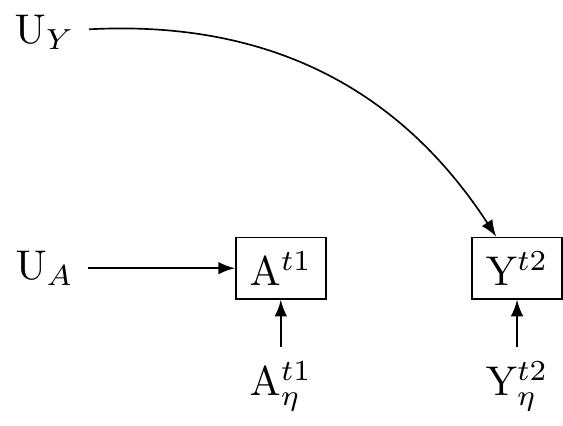
\includegraphics[width=0.6\textwidth,height=\textheight]{causal-dags_files/figure-pdf/fig-dag-uu-null-1.pdf}

}

\caption{\label{fig-dag-uu-null}Uncorrelated non-differential
measurement error does not bias estimates under the null, however may
attenuate true effects.}

\end{figure}

\hypertarget{uncorrelated-differential-directed-measurement-error}{%
\subsubsection{\texorpdfstring{2. \textbf{Uncorrelated differential
(directed) measurement
error}}{2. Uncorrelated differential (directed) measurement error}}\label{uncorrelated-differential-directed-measurement-error}}

As shown in Figure~\ref{fig-dag-indep-d-effect}, uncorrelated
differential (or directed) measurement error occurs when the errors in
measurement are related to the level of exposure or outcome, but not to
each other. For instance, societies with stronger `beliefs in Big Gods'
might cause a society to provide more or less detailed records of
`social complexity'. However, in the absence of any intervention on
beliefs in Gods, there is no association between the measurement errors.
Here, the errors are differential as they depend on the intensity of
religious beliefs, but uncorrelated as the errors in documenting
`beliefs in Big Gods' and `social complexity' are otherwise independent
of each other. Uncorrelated differential (or directed) measurement error
is presented in Figure~\ref{fig-dag-indep-d-effect} and leads to bias
under the null, indicated by the red path. Or equivalently, uncorrelated
differential (or directed) measurement error opens a back-door path
between the exposure and the outcome.

Note that the bias presented in Figure~\ref{fig-dag-indep-d-effect},
which is an example of directed measurement error, also describes the
bias we considered when there is panel attrition, and which the exposure
and affects selection (see: Figure~\ref{fig-dag-8-5}). In that scenario,
the outcome in the selected group is measured with error -- it no long
represents the measurement of the outcome in the source population at
baseline -- and further more, this error is affected by the exposure.
The previous example described bias in estimation from the vantage point
of collider stratification, however the example may be equally explained
from the more general vantage point of directed measurement bias.

\begin{figure}

{\centering 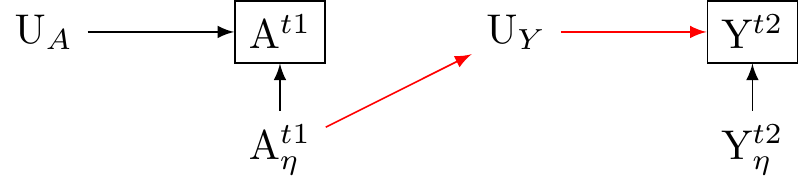
\includegraphics[width=1\textwidth,height=\textheight]{causal-dags_files/figure-pdf/fig-dag-indep-d-effect-1.pdf}

}

\caption{\label{fig-dag-indep-d-effect}Directed independent
(uncorrelated) measurement error biases effect estimates, indicated by
the red path. The selection bias presented in the previous graph is an
instance of directed independent measurement error.}

\end{figure}

\hypertarget{correlated-non-differential-undirected-measurement-error}{%
\subsubsection{\texorpdfstring{3. \textbf{Correlated non-differential
(undirected) measurement
error}}{3. Correlated non-differential (undirected) measurement error}}\label{correlated-non-differential-undirected-measurement-error}}

As shown Figure~\ref{fig-dag-dep-u-effect} correlated non-differential
(undirected) measurement error occurs when the errors in measuring both
the exposure and outcome are related to each other, but not to the level
of exposure or outcome. The scenario is presented in
Figure~\ref{fig-dag-dep-u-effect}. Imagine that some societies had more
advanced record-keeping systems that resulted in more accurate and
detailed accounts of both `beliefs in Big Gods' and `social complexity'
and furthermore that the record keepers provide better information about
religious beliefs. These errors between beliefs in Big Gods and social
complexity might be correlated because the accuracy of records on both
variables is influenced by the same underlying factor (the
record-keeping abilities), but they are non-differential insofar as true
religious beliefs and true social complexity do not affect bias in the
record keeping. Correlated non-differential measurement error may induce
bias under the null, indicated by the red path in
Figure~\ref{fig-dag-dep-u-effect}.

\begin{figure}

{\centering 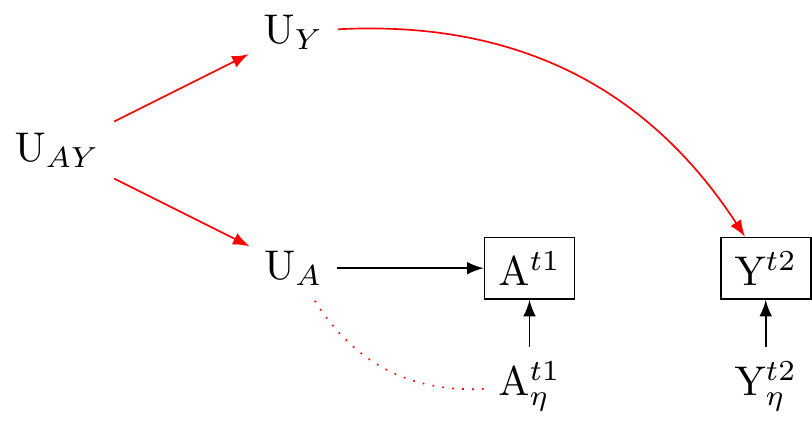
\includegraphics[width=0.8\textwidth,height=\textheight]{causal-dags_files/figure-pdf/fig-dag-dep-u-effect-1.pdf}

}

\caption{\label{fig-dag-dep-u-effect}Correlated undirected measurement
error can dilute the estimates of true effects, indicated by the red
path.}

\end{figure}

\hypertarget{correlated-differential-directed-measurement-error}{%
\subsubsection{\texorpdfstring{4. \textbf{Correlated differential
(directed) measurement
error}}{4. Correlated differential (directed) measurement error}}\label{correlated-differential-directed-measurement-error}}

Correlated differential (directed) measurement error occurs when the
errors in measurement are related to each other and also to the level of
exposure or outcome. This structural problem is presented in
Figure~\ref{fig-dag-d-d}. Suppose societies with stronger beliefs in Big
Gods tend to record both their religious beliefs and social structures
more meticulously, with this record-keeping being conducted by religious
elites. The errors may be both correlated and differential if societies
with beliefs in Big Gods tend to favour these religious elites, leading
to biased records.

Consider further the three-wave panel design where we aim to estimate
the effect of self-reported religious service attendance on
self-reported monthly donations to charity. A set of confounders is
included at baseline, comprising previous measures of religious service
attendance and monthly donations to charity. Because our measures rely
on self-reports they may be especially prone to measurement error.

Assume there is an unmeasured common cause affecting both the
measurement error of religious service attendance and the measurement
error of donations to charity. This might occur if individuals
consistently over- or under-report their religious service attendance
and donations due to social desirability bias.

In part 3, we discussed how including the exposure measured at baseline
can reduce confounding in a three-wave panel design. By controlling for
the baseline exposure, we effectively adjust for any static
characteristics that might cause correlation in both the exposure and
outcome.

Now for measurement error, including baseline measures could mitigate
the impact of these errors on causal effect estimation, provided the
errors are random and not systematically associated across time points.

To see this, let \(A_0\), \(A_1\) denote the exposure at baseline and
follow-up, and \(Y_0\), \(Y_1\) denote the outcome at baseline and
follow-up. The true values are denoted without primes, and the measured
values with primes. We assume the measurement error is additive:

\(A'_0 = A_0 + UA_0\),

\(A'_1 = A_1 + UA_1\),

\(Y'_0 = Y_0 + UY_0\),

\(Y'_2 = Y_2 + UY_2\),

where \(UA_0\), \(UA_1\) are the measurement errors for the exposure at
baseline and follow-up, and \(UY_0\), \(UY_2\) are the measurement
errors for the outcome at baseline and follow-up. If the errors are
correlated, then \(Cov(UA_0, UY_0) \neq 0\) and/or
\(Cov(UA_1, UY_2) \neq 0\).

In a model that includes \(A'_0\) and \(Y'_0\) as covariates, the
estimated effect of \(A'_1\) on \(Y'_2\) identifies the effect of change
in the exposure from baseline to follow-up on the change in the outcome
from baseline to follow-up. Because our interest is in this effect, we
control for the baseline exposure and outcome measures. This strategy
will mitigate bias arising from correlated errors if the following
conditions hold:

\(E(UA_0) = E(UA_1)\) and \(E(UY_0) = E(UY_2)\) (i.e., the expectation
of the measurement errors does not change over time),

\(Cov(UA_0, UY_2) = Cov(UA_1, UY_2)\) (i.e., the correlation between the
errors does not change over time).

Thus, including baseline measurements in our model can help to mitigate
undirected measurement error. However, this solution hinges on the
measurement error being directionless and non-differential with respect
to time. If the measurement error varies over time or with respect to
other variables in the model, baseline measurement control will be
inadequate for confounding control.

Consider a scenario where individuals who attend religious service more
at time 1 acquire greater social desirability bias, becoming more likely
to over-report socially desirable behaviours or under-report socially
undesirable ones. The structure of this scenario is presented in
Figure~\ref{fig-dag-d-d}. If the measured outcome at time 2 is
charitable giving, the increased social desirability bias could lead to
an over-estimation of the true level of giving. If we were to compare
reported charity at T2 with reported church attendance at T1, we might
falsely attribute the apparent increase in charity to the increase in
religious service, when in reality, the over-reporting arose from social
desirability bias. Thus, if the error of the outcome is affected by the
exposure, the causal effect of the increase in religious service on
giving might be different than it appears.

Thus, although controlling for baseline exposure is a powerful strategy
for isolating incidence effects and controlling confounding, we have
seen here that it is not a catch-all solution. Attention to the quality
of measures at all time points remains critical.

For instance, to avoid presentation bias, rather than asking whether one
has \emph{offered} help, we might ask whether one has \emph{received
help} -- under the assumption that if the community is more altruist
then the probability of receiving help will be higher.

\begin{figure}

{\centering 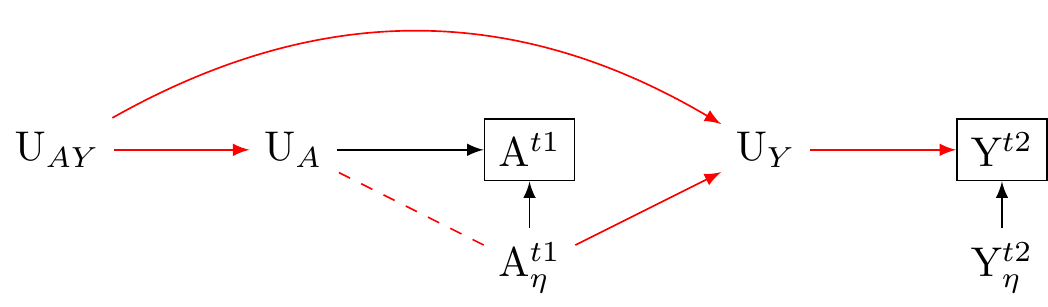
\includegraphics[width=1\textwidth,height=\textheight]{causal-dags_files/figure-pdf/fig-dag-d-d-1.pdf}

}

\caption{\label{fig-dag-d-d}Directed dependent (correlated) measurement
error biases effect estimates. Here, the exposure affects the
measurement error of the outcome. Additionally, the measurement errors
of the exposure and outcome are correlated. These dynamics open pathways
for bias.}

\end{figure}

\hypertarget{comparative-cultural-research-viewed-as-correlated-undirected-measurment-error}{%
\subsection{Comparative cultural research viewed as correlated
undirected measurment
error}\label{comparative-cultural-research-viewed-as-correlated-undirected-measurment-error}}

Against invariance testing, we should approach comparative research from
the vantage point of correlated measurement error. Amending
Figure~\ref{fig-dag-dep-u-effect}. Selecting on unmeasured correlated
error structures in the world we have
Figure~\ref{fig-dag-dep-u-effect-selection}.

Were we to select from a setting in which there was no systematic
(correlated) error structures between the measurements of the exposures
and the measurements of the outcomes we would avoid such confounding.

Note that it is not merely a matter of transporting results from the
sample population to another population. Rather, the act of selection
induces bias.

\begin{figure}

{\centering \includegraphics[width=1\textwidth,height=\textheight]{causal-dags_files/figure-pdf/fig-dag-dep-u-effect-selection-1.pdf}

}

\caption{\label{fig-dag-dep-u-effect-selection}Measurement bias in
comparative cross-cultural research}

\end{figure}

\hypertarget{casual-diagrams-clarify-the-structural-assumptions-underlying-classical-measurement-theory}{%
\subsection{Casual diagrams clarify the structural assumptions
underlying classical measurement
theory}\label{casual-diagrams-clarify-the-structural-assumptions-underlying-classical-measurement-theory}}

Researchers working in cultural evolution often incorporate multi-item
constructs into their panel study designs, a practice which is aligned
with the recommendations of conventional psychometric theory. However,
classical psychometric theory emerged without the benefit of causal
theories. As noted by Tyler VanderWeele, issues arise when evaluating
the causal assumptions of formative and reflective models
(\protect\hyperlink{ref-vanderweele2022}{\textbf{vanderweele2022?}}).
Let us first consider the issues before expanding on how they manifest
in panel research.

There are two prevailing approaches in this area: formative and
reflective models. The focus here will be on reflective models, though
it should be noted that the issues identified also apply to formative
models, as outlined by VanderWeele
{[}(\protect\hyperlink{ref-vanderweele2022}{\textbf{vanderweele2022?}}){]}\footnote{In
  a formative model, the observed variables are thought to cause the
  latent variable. As in the reflective model, there is a single latent
  variable. This latent variable, however, is considered the effect of
  the underlying indicators. In mathematical terms, if \(\eta\)
  represents the latent variable, \(\lambda_i\) denotes the weight for
  \(X_i\) (the observed variable), and \(\varepsilon\) is the error
  term, the latent variable \(\eta\) can be described as a composite of
  the observed variables \(X_i\), expressed as:
  \(\eta = \sum_i\lambda_i X_i\).}.

In a reflective model, researchers posit that a latent variable gives
rise to the observed indicators. Each observed variable (or indicator)
is seen as a `reflection' or manifestation of the latent variable. If
\(X_i\) is an observed variable (indicator), \(\lambda_i\) is the factor
loading for \(X_i\), \(\eta\) is the latent variable, and
\(\varepsilon_i\) is the error term associated with \(X_i\), the
reflective model can be formulated as:

\[X_i = \lambda_i \eta + \varepsilon_i\]

Factor analysis typically assumes a common latent variable, which is
responsible for the correlations observed among the indicators. The
causal assumptions linked to this concept are demonstrated in Figure
Figure~\ref{fig-dag-latent-1}.

\begin{figure}

{\centering 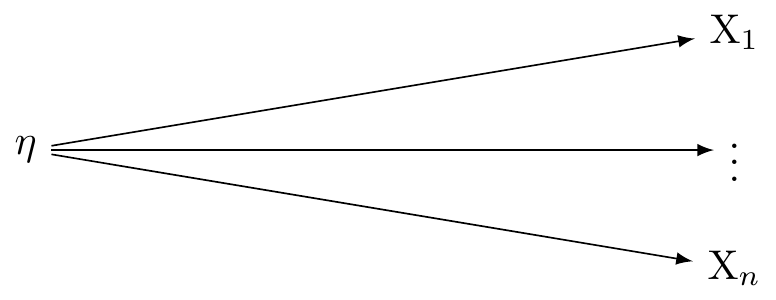
\includegraphics[width=0.6\textwidth,height=\textheight]{causal-dags_files/figure-pdf/fig-dag-latent-1-1.pdf}

}

\caption{\label{fig-dag-latent-1}Reflective model: assume univariate
latent variable η giving rise to indicators X1\ldots X3. Figure adapted
from VanderWeele: doi: 10.1097/EDE.0000000000001434}

\end{figure}

The statistical implications of the \textbf{reflective model} suggest
that the observed variables (indicators) are reflections or
manifestations of the latent variable, which is mathematically expressed
as \(X_i = \lambda_i \eta + \varepsilon_i\). The factor analytic
tradition goes one step further by proposing a structural assumption
that a univariate latent variable causally affects the observed
variables. Hence, the reflective model yields
\(X_i = \lambda_i \eta + \varepsilon_i\), which is assumed to underpin
the structural assumptions shown in Figure
Figure~\ref{fig-structural-assumptions-reflective-model}.

\begin{figure}

{\centering 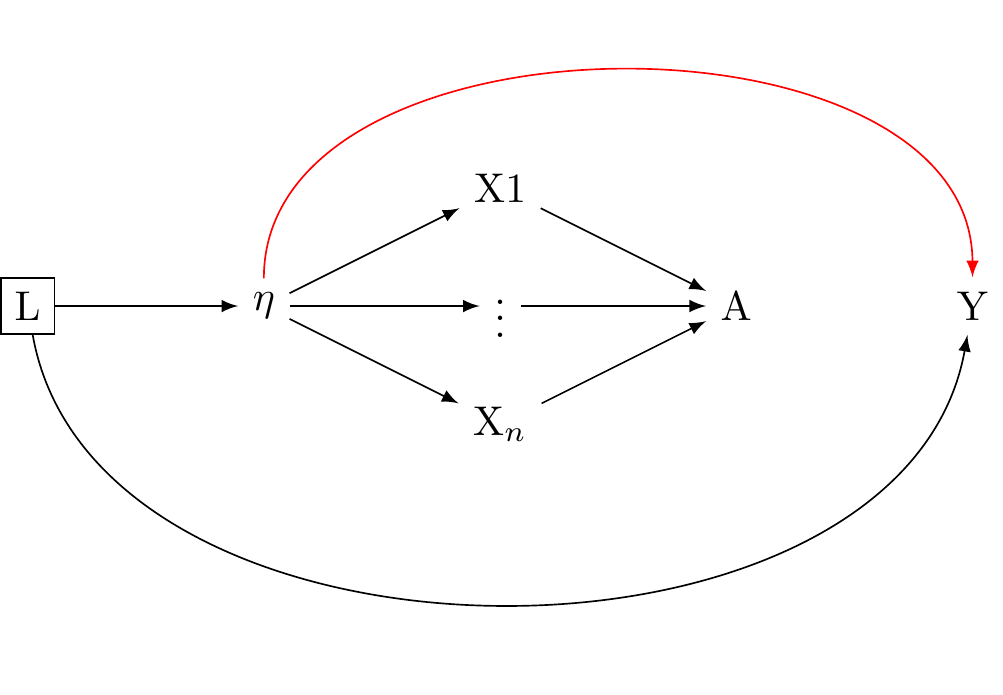
\includegraphics[width=0.8\textwidth,height=\textheight]{causal-dags_files/figure-pdf/fig-structural-assumptions-reflective-model-1.pdf}

}

\caption{\label{fig-structural-assumptions-reflective-model}Reflective
Model: causal assumptions. Figure adapted from VanderWeele: doi:
10.1097/EDE.0000000000001434}

\end{figure}

VanderWeele notices that while the statistical model
\(X_i = \lambda_i \eta + \varepsilon_i\) concurs with the structural
assumptions in Figure
Figure~\ref{fig-structural-assumptions-reflective-model}, it can also
align with various causal models. For instance, the statistical model is
compatible with the reality presented in @
fig\_dag\_multivariate\_reality\_again, where unique latent variables
give rise to distinct indicators, some of which (but not necessarily
all) have a causal effect on the outcome. The statistical model does not
provide clarity about which structural model is accurate. Additionally,
the assumption that a univariate underlying reality forms the basis of
the formative and reflective latent factor models, which is a much
stronger assumption than has been previously acknowledged in
psychometric literature. For widely used measures these assumptions fail
to withstand empirical scrutiny
(\protect\hyperlink{ref-vanderweele2022b}{\textbf{vanderweele2022b?}}).

\begin{figure}

{\centering 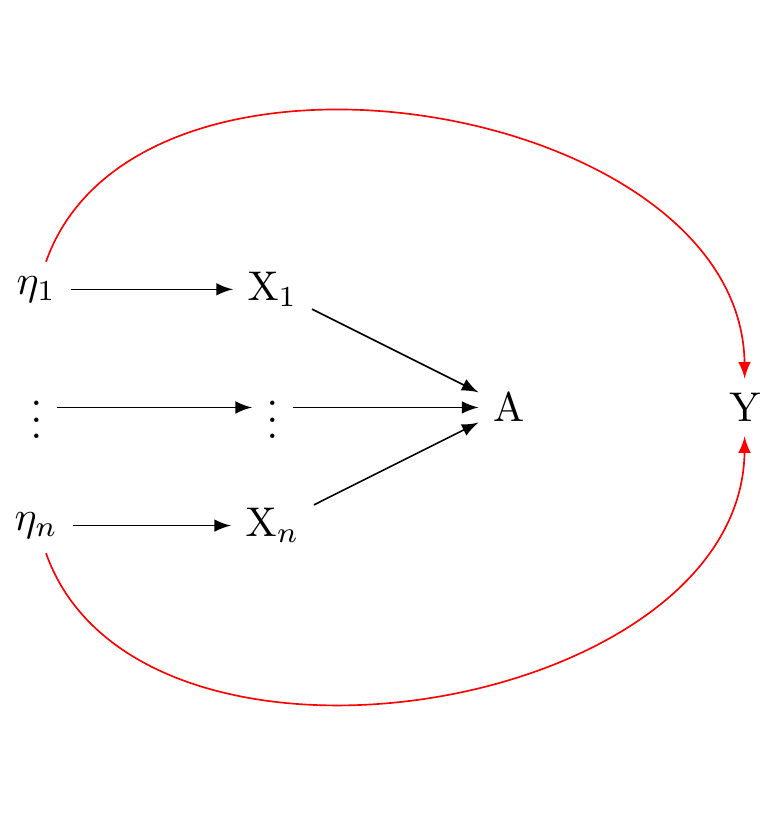
\includegraphics[width=0.6\textwidth,height=\textheight]{causal-dags_files/figure-pdf/fig_dag_multivariate_reality_again-1.pdf}

}

\caption{Multivariate reality gives rise to the indicators, from which
we draw our measures. Figure adapted from VanderWeele: doi:
10.1097/EDE.0000000000001434}

\end{figure}

VanderWeele suggests that construct measures can still be utilised in
applied research by extending the theory of causal inference under
multiple interventions to factor models
(\protect\hyperlink{ref-vanderweele2022a}{\textbf{vanderweele2022a?}})
(for a detailed discussion, refer to Appendix 1).

By expressing our measured variables as functions of indicators, and
assuming the true underlying reality as a coarsened measure of a
potentially complex latent reality, we can consistently estimate causal
effects under this extended theory. This approach is illustrated in
Figure~\ref{fig-dag-multiple-version-treatment-applied-measurement}.

\begin{figure}

{\centering 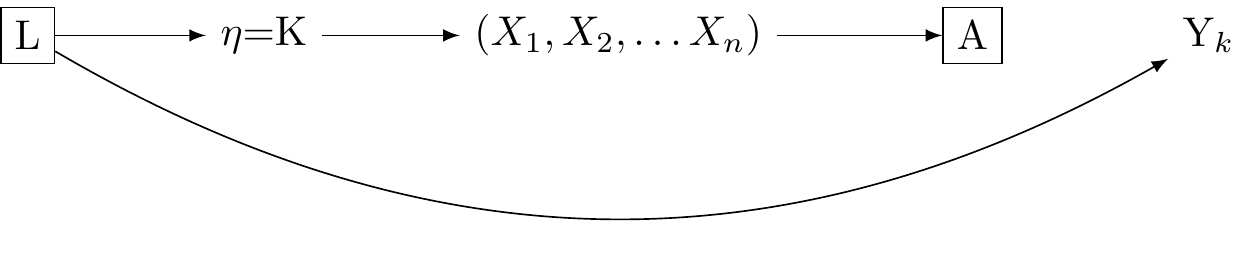
\includegraphics[width=0.8\textwidth,height=\textheight]{causal-dags_files/figure-pdf/fig-dag-multiple-version-treatment-applied-measurement-1.pdf}

}

\caption{\label{fig-dag-multiple-version-treatment-applied-measurement}Multiple
Versions of treatment applied to measuremen.Figure adapted from
VanderWeele: doi: 10.1097/EDE.0000000000001434}

\end{figure}

\hypertarget{causal-diagrammes-reveal-matters-are-worse-when-the-components-of-constructs-are-measured-withe-error.}{%
\subsection{Causal diagrammes reveal matters are worse when the
components of constructs are measured withe
error.}\label{causal-diagrammes-reveal-matters-are-worse-when-the-components-of-constructs-are-measured-withe-error.}}

Consider a three wave panel where, for simplicity, we assume no
unmeasured confounding is present. Our exposure \(A\) can be measured by
a function of indicators, denoted as \(A_{f(A_1, A_2, ..., A_n)}\),
forming a coarsened state from a multivariate reality. Each element of
this reality has a corresponding structural component, denoted as
\(\eta_{A_1}, \eta_{A_2}, ..., \eta_{A_n}\). These components are
measured with their respective error terms,
\(U\eta_{A_1}, U\eta_{A_2}, ..., U\eta_{A_n}\).

Similar to the exposure, our outcome Y can be conceptualised as a
function of indicators, \(Y_{f(Y_1, Y_2, ..., Y_n)}\), of a latent
reality. This reality is expressed through the latent components
\(\eta_{Y_1}, \eta_{Y_2}, ..., \eta_{Y_n}\), each having their
associated error term \(U\eta_{Y_1}, U\eta_{Y_2}, ..., U\eta_{Y_n}\).

Figure~\ref{fig-dag-coarsen-measurement-error} illustrates the assumed
reality. It shows possible paths for confounding via directed
measurement error. Each path is represented by a structural component
\(\eta_{A_n}\) and its associated error term \(U\eta_{Y_n}\). Here we
present three possible confounding paths that are possible from directed
measurement error.

Note that the potential for confounding arising from measurement error
in panel designs depends fundamentally on the particular relationships
and dependencies among variables, not merely their quantity. However, we
can see here that, theoretically, a larger number of latent states or
error terms could amplify the possibilities for confounding. In a
simplistic scenario, \emph{every} latent variable associated with an
exposure could affect each error term of an outcome, leading to an
expansive network of confounding paths.

This underscores thinking very carefully about the composite terms when
using psychological constructs. In many cases researchers might wish to
use single item measures. However, general rule here is not possible.
Every case must be considered with careful attention to the meanings of
the items, their likely interpretations, and their potential causal
underpinnings over time.

\begin{figure}

{\centering 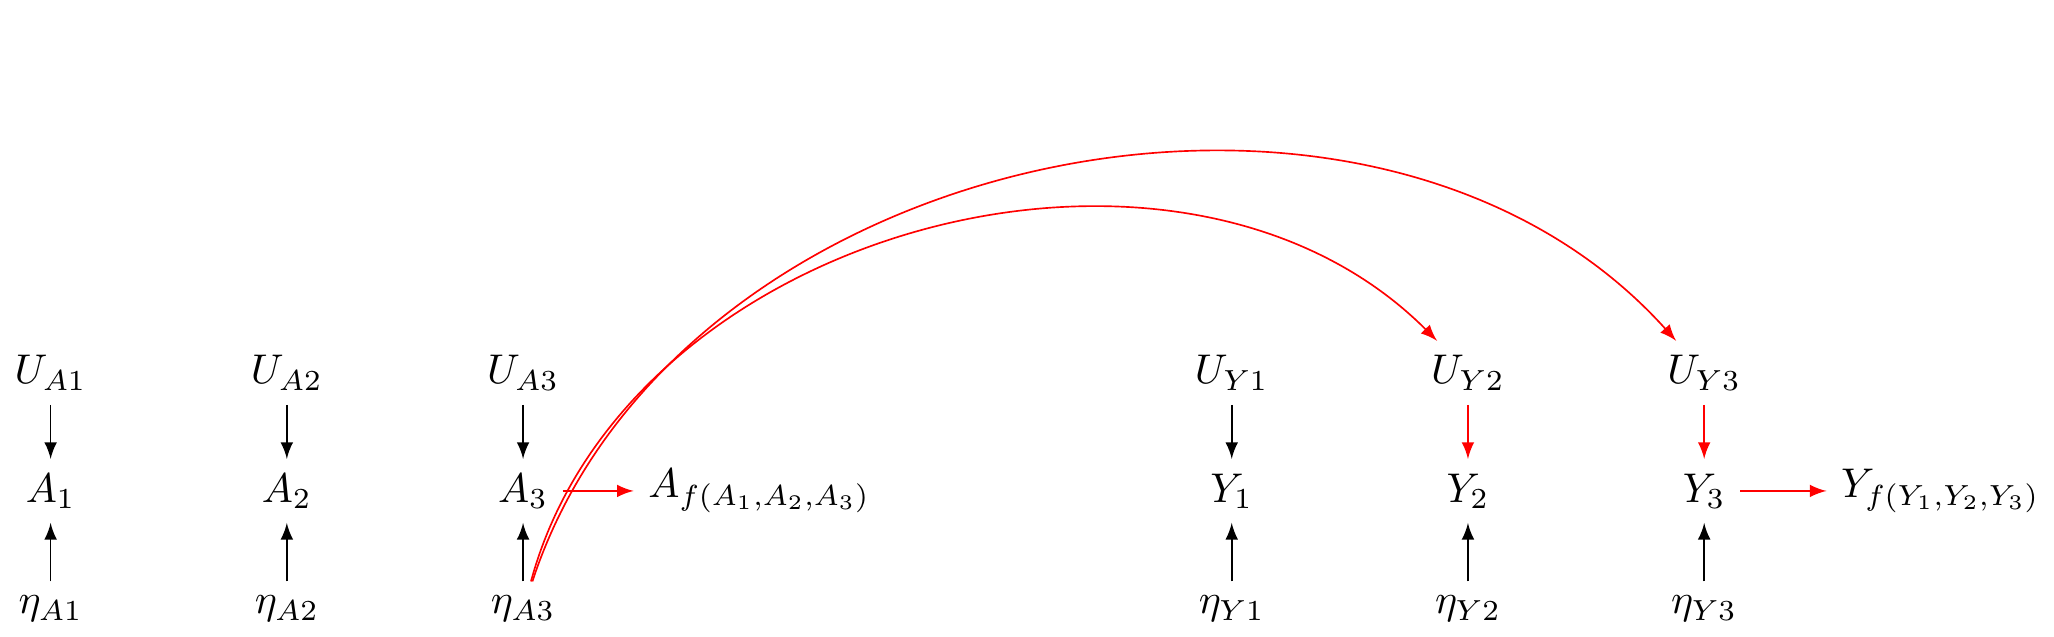
\includegraphics[width=1\textwidth,height=\textheight]{causal-dags_files/figure-pdf/fig-dag-coarsen-measurement-error-1.pdf}

}

\caption{\label{fig-dag-coarsen-measurement-error}Where there are many
indicators of a psychological construct, there are many opportunities
for additional confounding by directed measureemnt error.}

\end{figure}

\hypertarget{summary-part-5}{%
\subsection{Summary Part 5}\label{summary-part-5}}

In Part 5, the focus is on understanding measurement and confounding
errors in the three-wave panel design using causal diagrams. We discuss
four types of measurement errors and how they may affect research
results. These include uncorrelated non-differential (undirected)
measurement error, uncorrelated differential (directed) measurement
error, correlated non-differential (undirected) measurement error, and
correlated differential (directed) measurement error.

Within a three-wave panel design, I discussed an example where the
estimation of the effect of self-reported religious service attendance
on self-reported monthly donations to charity might be influenced by
systematic errors.

I emphasised that while adjusting for baseline exposure can help reduce
confounding and isolate incidence effects, it is not a solution for all
biases. Attention must be given to the quality of measurements at all
time points and the design of the questions to avoid potential biases,
such as presentation bias. causal diagrams are helpful in clarifying
these complex structures confounding.

\hypertarget{conclusions}{%
\subsection{Conclusions}\label{conclusions}}

\hypertarget{summary-of-advice}{%
\subsection{Summary of advice}\label{summary-of-advice}}

\begin{enumerate}
\def\labelenumi{\arabic{enumi}.}
\item
  \textbf{Define all variables clearly}: Ensure that all variables in
  your causal graph are distinctly defined.
\item
  \textbf{Define novel conventions}: if you are using unique conventions
  in your diagram, such as coloured arrows to indicate induced
  confounding, make sure to define them.
\item
  \textbf{Embrace minimalism}: include only the nodes and edges that
  clarify the problem at hand. Diagrams should be used when they provide
  clarity beyond what can be achieved by textual descriptions alone.
  That clarity is enhance by drawing only as much complexity as is
  needed to identify sources of counfounding and develop strategies for
  minimising bias.
\item
  \textbf{Ensure the graph is Acyclic}
\item
  \textbf{Maintain chronological order in the spatial organisation}:
  organise nodes in temporal sequence, usually from left to right or top
  to bottom. If depicting repeated measures, use time subscripts for
  clarity.
\end{enumerate}

\emph{Note that chronologically ordered causal diagrams are ordinary
causal diagrams whose spatial properties help to improve strategies for
addressing bias in causal estimation.} They are not structurally
different from non-chronologically ordered causal diagrams. However, we
shall see that by maintaining chronological order we may greatly enhance
the effectiveness of the tool.

\begin{enumerate}
\def\labelenumi{\arabic{enumi}.}
\setcounter{enumi}{5}
\item
  \textbf{Generally, time-stamp your nodes}: it is often useful to
  time-stamp nodes for clearer temporal understanding, for example,
  \(L_{t0} \rightarrow A_{t1} \rightarrow Y_{t2}\).
\item
  \textbf{Included nodes for unmeasured confounding}: when exposures are
  not assigned randomly, assume the existence of unmeasured confounding.
  Plan for sensitivity analyses to gauge the impact of unmeasured
  confounding on your findings.
\item
  \textbf{Include nodes for selection}: when applicable, include nodes
  for selection variables. This helps to understand potential sources of
  selection bias in your study.
\item
  \textbf{Consider mediators and interactions}: when mediation or
  interaction is of interest, these should be appropriately represented
  in the diagram. However, be mindful not to attempt to represent
  non-linear relationships graphically.
\item
  \textbf{Appreciate the qualitative role of causal diagrams}: remember,
  causal diagrams serve as qualitative visual tools rather than
  quantitative models. When strategies like time stamps are implemented,
  they are used for maintaining sufficient clarity in chronological
  order needed to understand potential confounding. They need not denote
  specific time intervals. Again we should aim for simplicity in our
  causal DAGs - include only the level of detail necessary to elucidate
  strategies for controlling confounding.
\item
  \textbf{Measurement error} It is generally important to include
  measurement error on the graph.
\end{enumerate}

Topics not covered:

\begin{enumerate}
\def\labelenumi{\arabic{enumi}.}
\tightlist
\item
  \textbf{Signed edges}
\item
  \textbf{SWIGS}
\item
  \textbf{Need for time -- comment on funding}
\end{enumerate}

\hypertarget{stray-points-to-address}{%
\subsection{Stray points to address}\label{stray-points-to-address}}

\begin{enumerate}
\def\labelenumi{\arabic{enumi}.}
\tightlist
\item
  Structural equation models are not causal diagrams
\item
  causal diagrams are non-parametric
\item
  causal diagrams represent interactions \(A \to Y \leftarrow B\) (two
  arrows into the outcome)
\item
  We may distinguish between effect modification and interaction.
\end{enumerate}

\hypertarget{else-for-conclusion}{%
\subsection{ELSE (for conclusion)}\label{else-for-conclusion}}

\begin{itemize}
\tightlist
\item
  Where possible do experiments, but we cannot always perform
  experiments
\item
  No multi-level models
\item
  Don't report regression coefficients.
\item
  Good measures
\item
  Retention
\item
  Check positivity -- how many change.
\item
  (causation not all of science)
\item
  (need for assumpitions)
\item
  Causal estimation is not all of science. And it is not all of
  causality.
\item
  Curse of dimensionality
\item
  Tracking change
\item
  Again, \emph{counterfactual data-science}.
\end{itemize}

\hypertarget{appendix-1-review-of-the-theory-of-multiple-versions-of-treatment}{%
\section{Appendix 1: Review of the theory of multiple versions of
treatment}\label{appendix-1-review-of-the-theory-of-multiple-versions-of-treatment}}

\begin{figure}

{\centering 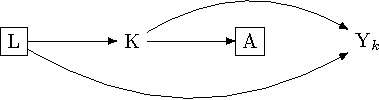
\includegraphics[width=1\textwidth,height=\textheight]{causal-dags_files/figure-pdf/fig_dag_multiple_version_treatment_dag-1.pdf}

}

\caption{Multiple Versions of treatment. Heae, A is regarded to bbe a
coarseneed version of K}

\end{figure}

Perhaps not all is lost. VanderWeele looks to the theory of multiple
versions of treatment for solace.

Recall, a causal effect is defined as the difference in the expected
potential outcome when everyone is exposed (perhaps contrary to fact) to
one level of a treatment, conditional on their levels of a confounder,
with the expected potential outcome when everyone is exposed to a a
different level of a treatement (perhaps contrary to fact), conditional
on their levels of a counfounder.

\[ \delta = \sum_l \left( \mathbb{E}[Y|A=a,l] - \mathbb{E}[Y|A=a^*,l] \right) P(l)\]

where \(\delta\) is the causal estimand on the difference scale
\((\mathbb{E}[Y^0 - Y^0])\).

In causal inference, the multiple versions of treatment theory allows us
to handle situations where the treatment isn not uniform, but instead
has several variations. Each variation or ``version'' of the treatment
can have a different effect on the outcome. However, consistency is not
violated because it is redefined: for each version of the treatment, the
outcome under that version is equal to the observed outcome when that
version is received. Put differently we may think of the indicator \(A\)
as corresponding to many version of the true treament \(K\). Where
conditional independence holds such that there is a absence of
confounding for the effect of \(K\) on \(Y\) given \(L\), we have:
\(Y(k)\coprod A|K,L\). This states conditional on \(L\), \(A\) gives no
information about \(Y\) once \(K\) and \(L\) are accounted for. When
\(Y = Y(k)\) if \(K = k\) and Y\((k)\) is independent of \(K\),
condition on \(L\), then \(A\) may be thought of as a coarsened
indicator of \(K\), as shown in
(\protect\hyperlink{ref-fig_dag_multiple_version_treatment_dag}{\textbf{fig\_dag\_multiple\_version\_treatment\_dag?}})
We may estimate consistent causal effects where:

\[ \delta = \sum_{k,l} \mathbb{E}[Y(k)|l] P(k|a,l) P(l) - \sum_{k,l} \mathbb{E}[Y(k)|l] P(k|a^*,l) P(l)\]

The scenario represents a hypothetical randomised trial where within
strata of covariates \(L\), individuals in one group receive a treatment
\(K\) version randomly assigned from the distribution of \(K\)
distribution \((A = 1, L = l)\) sub-population. Meanwhile, individuals
in the other group receive a randomly assigned \(K\) version from
\((A = 0, L = l)\)

This theory finds its utility in scenarios where treatments seldom
resemble each other (see: (\protect\hyperlink{ref-vanderweele2013}{Tyler
J. VanderWeele and Hernan 2013})).

\hypertarget{references}{%
\section*{References}\label{references}}
\addcontentsline{toc}{section}{References}

\hypertarget{refs}{}
\begin{CSLReferences}{1}{0}
\leavevmode\vadjust pre{\hypertarget{ref-barrett2021}{}}%
Barrett, Malcolm. 2021. \emph{Ggdag: Analyze and Create Elegant Directed
Acyclic Graphs}. \url{https://CRAN.R-project.org/package=ggdag}.

\leavevmode\vadjust pre{\hypertarget{ref-basten2013}{}}%
Basten, Christoph, and Frank Betz. 2013. {``Beyond Work Ethic: Religion,
Individual, and Political Preferences.''} \emph{American Economic
Journal: Economic Policy} 5 (3): 67--91.
\url{https://doi.org/10.1257/pol.5.3.67}.

\leavevmode\vadjust pre{\hypertarget{ref-becker2016}{}}%
Becker, Sascha O, Steven Pfaff, and Jared Rubin. 2016. {``Causes and
Consequences of the Protestant Reformation.''} \emph{Explorations in
Economic History} 62: 125.

\leavevmode\vadjust pre{\hypertarget{ref-bulbulia2022}{}}%
Bulbulia, Joseph A. 2022. {``A Workflow for Causal Inference in
Cross-Cultural Psychology.''} \emph{Religion, Brain \& Behavior} 0 (0):
1--16. \url{https://doi.org/10.1080/2153599X.2022.2070245}.

\leavevmode\vadjust pre{\hypertarget{ref-cinelli2022}{}}%
Cinelli, Carlos, Andrew Forney, and Judea Pearl. 2022. {``A Crash Course
in Good and Bad Controls.''} \emph{Sociological Methods \& Research},
May, 00491241221099552. \url{https://doi.org/10.1177/00491241221099552}.

\leavevmode\vadjust pre{\hypertarget{ref-collinson2007}{}}%
Collinson, Patrick. 2007. \emph{The Reformation: A History}. Vol. 19.
Modern Library.

\leavevmode\vadjust pre{\hypertarget{ref-edwards2015}{}}%
Edwards, Jessie K, Stephen R Cole, and Daniel Westreich. 2015. {``All
Your Data Are Always Missing: Incorporating Bias Due to Measurement
Error into the Potential Outcomes Framework.''} \emph{International
Journal of Epidemiology} 44 (4): 14521459.

\leavevmode\vadjust pre{\hypertarget{ref-gawthrop1984}{}}%
Gawthrop, Richard, and Gerald Strauss. 1984. {``Protestantism and
Literacy in Early Modern Germany.''} \emph{Past \& Present}, no. 104:
3155.

\leavevmode\vadjust pre{\hypertarget{ref-greenland1999}{}}%
Greenland, S., J. Pearl, and J. M. Robins. 1999. {``Causal diagrams for
epidemiologic research.''} \emph{Epidemiology (Cambridge, Mass.)} 10
(1): 37--48.

\leavevmode\vadjust pre{\hypertarget{ref-hernuxe1nmarobinsjm2020}{}}%
Hernán, MA, Robins JM. 2020a. \emph{Causal Inference: What If}. Boca
Raton: Chapman \& Hall/CRC.
\url{https://cdn1.sph.harvard.edu/wp-content/uploads/sites/1268/2021/03/ciwhatif_hernanrobins_30mar21.pdf}.

\leavevmode\vadjust pre{\hypertarget{ref-hernuxe1nmarobinsjm2020a}{}}%
---------. 2020b. \emph{Causal Inference: What If}. Boca Raton: Chapman
\& Hall/CRC.
\url{https://cdn1.sph.harvard.edu/wp-content/uploads/sites/1268/2021/03/ciwhatif_hernanrobins_30mar21.pdf}.

\leavevmode\vadjust pre{\hypertarget{ref-holland1986}{}}%
Holland, Paul W. 1986. {``Statistics and Causal Inference.''}
\emph{Journal of the American Statistical Association} 81 (396): 945960.

\leavevmode\vadjust pre{\hypertarget{ref-hume1902}{}}%
Hume, David. 1902. \emph{Enquiries Concerning the Human Understanding:
And Concerning the Principles of Morals}. Clarendon Press.

\leavevmode\vadjust pre{\hypertarget{ref-lewis1973}{}}%
Lewis, David. 1973. {``Causation.''} \emph{The Journal of Philosophy} 70
(17): 556--67. \url{https://doi.org/10.2307/2025310}.

\leavevmode\vadjust pre{\hypertarget{ref-mcelreath2020}{}}%
McElreath, Richard. 2020. \emph{Statistical Rethinking: A Bayesian
Course with Examples in r and Stan}. CRC press.

\leavevmode\vadjust pre{\hypertarget{ref-nalle1987}{}}%
Nalle, Sara T. 1987. {``Inquisitors, Priests, and the People During the
Catholic Reformation in Spain.''} \emph{The Sixteenth Century Journal},
557587.

\leavevmode\vadjust pre{\hypertarget{ref-pearl2009}{}}%
Pearl, Judea. 2009. {``Causal Inference in Statistics: An Overview.''}
\url{https://doi.org/10.1214/09-SS057}.

\leavevmode\vadjust pre{\hypertarget{ref-pearl2018}{}}%
Pearl, Judea, and Dana Mackenzie. 2018. \emph{The Book of Why: The New
Science of Cause and Effect}. Basic books.

\leavevmode\vadjust pre{\hypertarget{ref-robins1986}{}}%
Robins, James. 1986. {``A New Approach to Causal Inference in Mortality
Studies with a Sustained Exposure Period{\textemdash}application to
Control of the Healthy Worker Survivor Effect.''} \emph{Mathematical
Modelling} 7 (9): 1393--1512.
\url{https://doi.org/10.1016/0270-0255(86)90088-6}.

\leavevmode\vadjust pre{\hypertarget{ref-robins}{}}%
Robins, James M, and Miguel A Hernán. n.d. {``Estimation of the Causal
Effects of Time-Varying Exposures.''}

\leavevmode\vadjust pre{\hypertarget{ref-rohrer2018}{}}%
Rohrer, Julia M. 2018. {``Thinking Clearly about Correlations and
Causation: Graphical Causal Models for Observational Data.''}
\emph{Advances in Methods and Practices in Psychological Science} 1 (1):
2742.

\leavevmode\vadjust pre{\hypertarget{ref-rubin1976}{}}%
Rubin, D. B. 1976. {``Inference and Missing Data.''} \emph{Biometrika}
63 (3): 581--92. \url{https://doi.org/10.1093/biomet/63.3.581}.

\leavevmode\vadjust pre{\hypertarget{ref-suzuki2020}{}}%
Suzuki, Etsuji, Tomohiro Shinozaki, and Eiji Yamamoto. 2020. {``Causal
Diagrams: Pitfalls and Tips.''} \emph{Journal of Epidemiology} 30 (4):
153--62. \url{https://doi.org/10.2188/jea.JE20190192}.

\leavevmode\vadjust pre{\hypertarget{ref-swanson1967}{}}%
Swanson, Guy E. 1967. {``Religion and Regime: A Sociological Account of
the Reformation.''}

\leavevmode\vadjust pre{\hypertarget{ref-swanson1971}{}}%
Swanson, Guy E. 1971. {``Interpreting the Reformation.''} \emph{The
Journal of Interdisciplinary History} 1 (3): 419446.
\url{http://www.jstor.org/stable/202620}.

\leavevmode\vadjust pre{\hypertarget{ref-vanderweele2009}{}}%
VanderWeele, Tyler J. 2009. {``Concerning the Consistency Assumption in
Causal Inference.''} \emph{Epidemiology} 20 (6): 880.
\url{https://doi.org/10.1097/EDE.0b013e3181bd5638}.

\leavevmode\vadjust pre{\hypertarget{ref-vanderweele2018}{}}%
---------. 2018. {``On Well-Defined Hypothetical Interventions in the
Potential Outcomes Framework.''} \emph{Epidemiology} 29 (4): e24.
\url{https://doi.org/10.1097/EDE.0000000000000823}.

\leavevmode\vadjust pre{\hypertarget{ref-vanderweele2013}{}}%
VanderWeele, Tyler J, and Miguel A Hernan. 2013. {``Causal Inference
Under Multiple Versions of Treatment.''} \emph{Journal of Causal
Inference} 1 (1): 120.

\leavevmode\vadjust pre{\hypertarget{ref-weber1905}{}}%
Weber, Max. 1905. \emph{The Protestant Ethic and the Spirit of
Capitalism: And Other Writings}. Penguin.

\leavevmode\vadjust pre{\hypertarget{ref-weber1993}{}}%
---------. 1993. \emph{The Sociology of Religion}. Beacon Press.

\leavevmode\vadjust pre{\hypertarget{ref-westreich2010}{}}%
Westreich, Daniel, and Stephen R. Cole. 2010. {``Invited commentary:
positivity in practice.''} \emph{American Journal of Epidemiology} 171
(6). \url{https://doi.org/10.1093/aje/kwp436}.

\leavevmode\vadjust pre{\hypertarget{ref-westreich2015}{}}%
Westreich, Daniel, Jessie K Edwards, Stephen R Cole, Robert W Platt,
Sunni L Mumford, and Enrique F Schisterman. 2015. {``Imputation
Approaches for Potential Outcomes in Causal Inference.''}
\emph{International Journal of Epidemiology} 44 (5): 17311737.

\leavevmode\vadjust pre{\hypertarget{ref-wright1920}{}}%
Wright, Sewall. 1920. {``The Relative Importance of Heredity and
Environment in Determining the Piebald Pattern of Guinea-Pigs.''}
\emph{Proceedings of the National Academy of Sciences of the United
States of America} 6 (6): 320.

\leavevmode\vadjust pre{\hypertarget{ref-wright1923}{}}%
---------. 1923. {``The Theory of Path Coefficients a Reply to Niles's
Criticism.''} \emph{Genetics} 8 (3): 239.

\end{CSLReferences}



\end{document}
